\chapter[Diseño del software]{Diseño del software\label{cap:software}}

El software del prototipo se diseña como una cadena integrada de adquisición,
análisis, persistencia y visualización. A partir de imágenes solares y reportes
observacionales históricos se construyen conjuntos de entrenamiento trazables;
sobre ellos se entrena una arquitectura en cascada de inteligencia artificial para localizar y
clasificar regiones activas; los resultados se complementan con modelos
predictivos de evolución temporal; finalmente, la información generada se
almacena en una base de datos relacional y se expone mediante una plataforma web.

Esta organización mantiene una separación clara entre las funciones de
entrenamiento, inferencia, predicción y consulta, pero las conecta mediante los
mismos identificadores, fechas de observación, metadatos y otros elementos derivados.
De este modo, cada captura puede seguirse desde su origen visual hasta su
clasificación, almacenamiento y presentación.

\section{Datos de entrenamiento}

\label{sec:data-software}

Los datos de entrenamiento se obtienen a partir de dos fuentes
complementarias: imágenes de disco solar completo provenientes de SDO/HMI y
reportes diarios NOAA SRD, sigla utilizada para referirse a \textit{Solar Region
Summary}, correspondientes al período de 2010 al 2025
\citep{scherrer2012hmi,noaaSRS}. El acoplamiento entre ambas fuentes asocia,
para cada fecha, la evidencia visual del disco solar con la información
descriptiva de las regiones activas reportadas, incluyendo posición,
identificación NOAA y descriptores morfológicos. Esta fusión imagen--metadatos
permite generar etiquetas consistentes, trazables y útiles para entrenamiento
supervisado.

Aunque el sistema final está orientado a operar con imágenes en luz blanca, la
etapa de entrenamiento se apoyó en el acoplamiento HMI--SRD debido a que todos
los registros considerados corresponden a observaciones diarias de las
00:30~UTC. No se utilizaron capturas en luz blanca del SIDC para construir las
etiquetas de entrenamiento, ya que dicho repositorio no dispone de imágenes
sistemáticas en ese horario. La decisión es razonable desde el punto de vista
morfológico: ambas modalidades representan la fotosfera y muestran las manchas
solares como estructuras oscuras sobre el disco. La
Figura~\ref{fig:hmi-white-light-comparison} ilustra esta correspondencia visual
\citep{scherrer2012hmi,bobra2014sharp,zhou2023mcintosh,noaaSRS}.

\begin{figure}[H]
    \centering
    \begin{subfigure}[t]{0.47\textwidth}
        \centering
        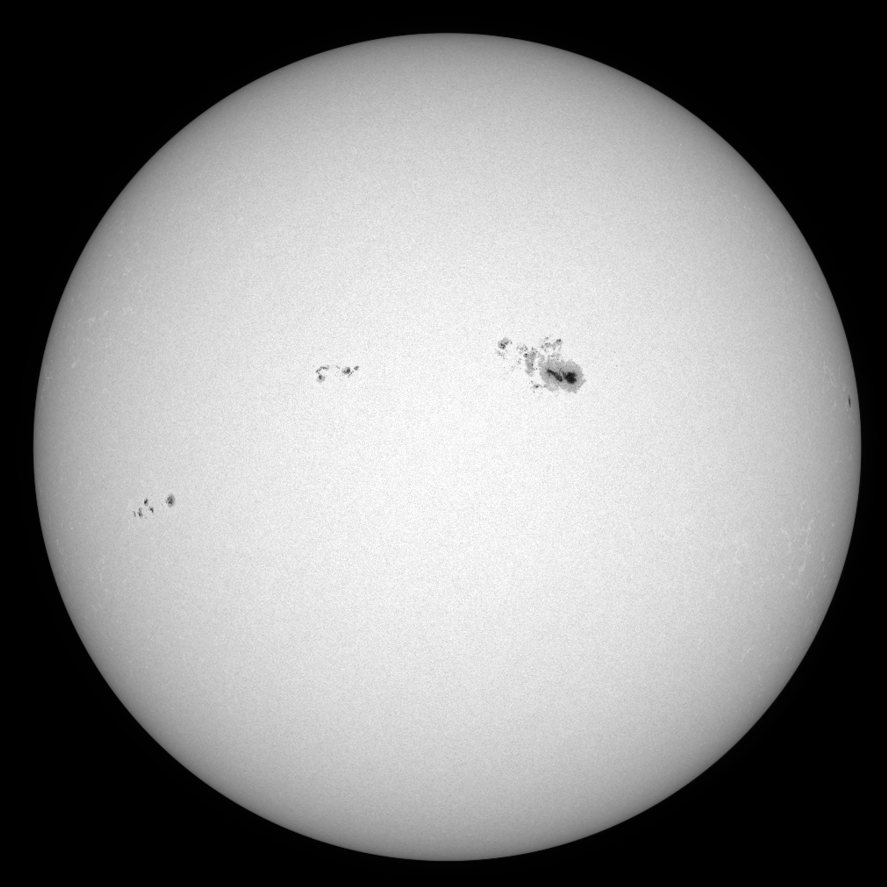
\includegraphics[width=\textwidth]{figures/data/hmi.png}
        \caption{Imagen HMI.}
    \end{subfigure}
    \hfill
    \begin{subfigure}[t]{0.47\textwidth}
        \centering
        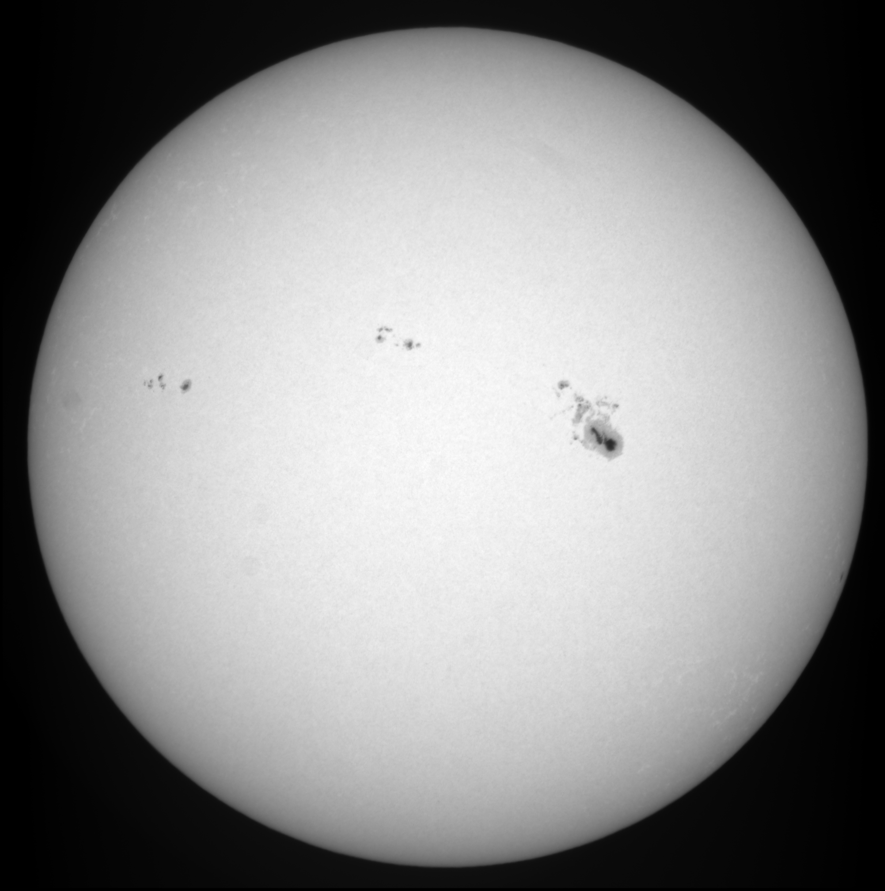
\includegraphics[width=\textwidth]{figures/data/wl.png}
        \caption{Imagen luz blanca.}
    \end{subfigure}
    \caption{Comparación visual entre modalidades fotosféricas de disco completo
    para la fecha 05-06-2025. La subfigura (a) corresponde a una imagen HMI
    obtenida por SDO/NASA, mientras que la subfigura (b) corresponde a una imagen
    luz blanca del SIDC del Royal Observatory of Belgium. \textbf{Fuente:} Elaboración propia a partir de imágenes SDO/NASA y SIDC.}
    \label{fig:hmi-white-light-comparison}
\end{figure}

\subsection{Transferencia de dominio y acoplamiento SDO--NOAA}

La transferencia de dominio se plantea como una estrategia para construir
etiquetas de entrenamiento a partir de fuentes observacionales complementarias.
Las imágenes SDO/HMI aportan una representación fotosférica uniforme del disco
solar completo, mientras que los reportes diarios NOAA SRD proporcionan la
identificación de regiones activas, sus coordenadas heliográficas y su
clasificación morfológica. El acoplamiento entre ambas fuentes permite trasladar
la información tabular de los reportes NOAA hacia posiciones concretas dentro de
cada imagen SDO/HMI.

En este flujo, cada fecha de observación funciona como clave temporal de enlace.
Primero se recupera la imagen HMI correspondiente a la observación diaria de las
00:30~UTC; luego se extraen del reporte NOAA SRD las regiones activas reportadas
para esa misma fecha, incluyendo número NOAA, latitud, longitud, extensión, área
y componentes de la clasificación Zurich--McIntosh. Posteriormente, las
coordenadas heliográficas se proyectan sobre el disco observado para ubicar cada
región en píxeles y generar anotaciones compatibles con las etapas de detección
y clasificación.

De este modo, la transferencia de dominio no se utiliza en esta sección como una
comparación operacional entre instrumentos, sino como un mecanismo de
etiquetado: las imágenes SDO/HMI constituyen el soporte visual y los registros
NOAA SRD aportan la semántica observacional. La combinación imagen--registro
permite construir ejemplos supervisados trazables, donde cada recorte conserva
su fecha, identificación NOAA, posición solar y etiqueta Zurich--McIntosh.

El preprocesamiento se orienta a reducir variaciones instrumentales y geométricas
que no forman parte de la morfología de interés. Se consideran la estimación del
área aparente, la proyección heliográfica para ubicar correctamente regiones
sobre el disco y transformaciones de realce local, incluyendo filtros tipo
\textit{black-hat} para destacar estructuras oscuras compactas frente al fondo
fotosférico. Estas operaciones no sustituyen al aprendizaje profundo; actúan como
una etapa de normalización que facilita la construcción de conjuntos de datos más
coherentes \citep{sayez2023sunscc,cesarHeliographic}.

La proyección heliográfica se formula a partir de la geometría esférica entre el
observador, el centro aparente del disco y la región activa. La
Figura~\ref{fig:heliographic-geometry-sw} resume la notación angular empleada,
mientras que la Figura~\ref{fig:heliographic-projection-sw} muestra un ejemplo de
proyección sobre una imagen SDO/HMI con retícula heliográfica y regiones NOAA SRD
superpuestas. En la implementación práctica, los cálculos astronómicos se
realizan con \texttt{SkyCoord} de \texttt{astropy.coordinates}, lo que permite
expresar posiciones en marcos consistentes, recuperar la geometría observacional
del Sol y obtener el ángulo heliográfico $B_0$ requerido por la transformación.

\begin{figure}[H]
    \centering
    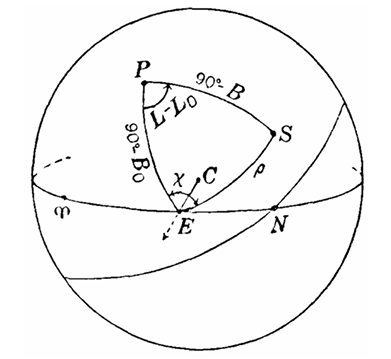
\includegraphics[width=0.44\textwidth]{figures/solar/helio_geom.png}
    \caption{Esquema geométrico de la proyección heliográfica. Se indican la
    latitud heliográfica $B$, la longitud relativa $L-L_0$, la distancia angular
    central $\rho$, el ángulo posicional $\theta$ y la inclinación heliográfica
    $B_0$ del eje solar respecto del observador. \textbf{Fuente:} adaptado de
    \textit{CESAR's Booklet} de la ESA.}
    \label{fig:heliographic-geometry-sw}
\end{figure}

\begin{figure}[H]
    \centering
    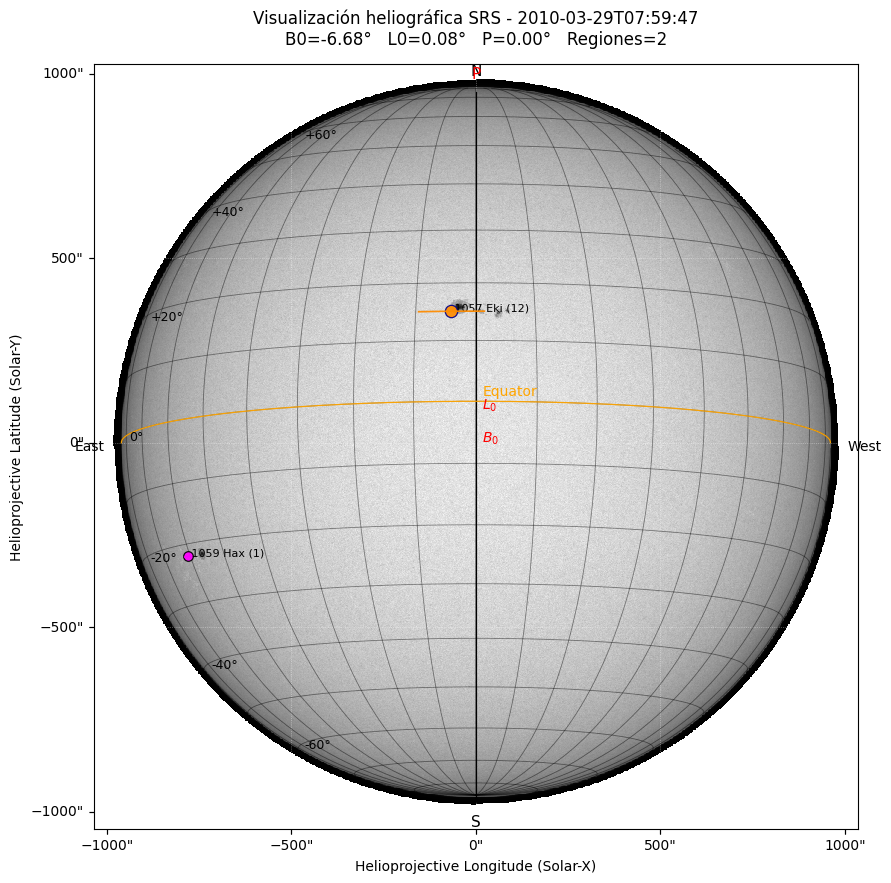
\includegraphics[width=0.8\textwidth]{figures/solar/helio_proj.png}
    \caption{Ejemplo de proyección heliográfica sobre una imagen SDO/HMI con
    retícula solar, ecuador proyectado y regiones activas asociadas al contenido
    NOAA SRD. La visualización permite verificar la coherencia entre posiciones
    heliográficas, latitudes proyectadas y etiquetas morfológicas. \textbf{Fuente:} Elaboración propia.}
    \label{fig:heliographic-projection-sw}
\end{figure}

Siguiendo la formulación geométrica de coordenadas heliográficas, la relación
entre la distancia radial observada $r$, el radio aparente del disco $r_0$ y el
ángulo auxiliar $\psi$ se expresa como
\begin{equation}
\psi = \frac{\alpha}{2}\,\frac{r}{r_0},
\end{equation}
donde $\alpha$ es el diámetro angular aparente del Sol. Bajo la aproximación de
ángulos pequeños, la distancia angular central respecto del centro del disco se
obtiene mediante
\begin{equation}
\rho = \arcsin\!\left(\frac{\psi}{\alpha/2}\right) - \psi.
\end{equation}
Si $(x,y)$ denotan las coordenadas cartesianas de la región activa medidas
respecto del centro del disco, el ángulo posicional se calcula como
\begin{equation}
\theta = \arctan\!\left(\frac{x}{y}\right).
\end{equation}
Conocidos $B_0$, $\rho$ y $\theta$, la latitud heliográfica $B$ queda dada por
\begin{equation}
\sin(B) = \sin(B_0)\cos(\rho) + \cos(B_0)\sin(\rho)\cos(\theta),
\end{equation}
mientras que la longitud heliográfica se recupera a partir de
\begin{equation}
L = \arcsin\!\big(\sin(\rho)\sin(\theta)\cos(B)\big) + L_0,
\end{equation}
donde $L_0$ representa la longitud del meridiano central. Estas ecuaciones
permiten trasladar detecciones en píxeles hacia coordenadas heliográficas antes
de asociarlas con las entradas NOAA SRD \citep{cesarHeliographic,noaaSRS}.

Se generaron dos colecciones diferenciadas. DB1 contiene aproximadamente 4700
imágenes de disco completo de tamaño 1024\,$\times$\,1024 con cajas delimitadoras
asociadas a grupos solares; se utiliza para entrenar el detector. DB2 contiene
alrededor de 15000 recortes derivados de dichas regiones y reinsertados en un
lienzo de 224\,$\times$\,224, preservando proporciones para evitar distorsiones
severas durante el redimensionamiento. DB2 se destina a la clasificación
Zurich--McIntosh.

La construcción de DB2.1 se apoya en una cadena de refinamiento donde el
detector YOLO26n, entrenado sobre DB1, se aplica sobre imágenes preprocesadas
mediante segmentación determinista y realce con filtro \textit{black-hat}. Aunque
el modelo se presenta formalmente en la Sección~\ref{sec:training}, se menciona
en este apartado porque participa en una iteración complementaria sobre los datos
de DB2: sus detecciones permiten ajustar la ubicación de las regiones candidatas,
reconstruir los recortes y obtener una versión DB2.1 con mejor correspondencia
entre imagen, posición y etiqueta. Las regiones candidatas se asocian luego con
el contenido diario de NOAA SRD para recuperar identidad, posición y etiqueta
morfológica, lo que permite generar recortes más consistentes para la
clasificación \citep{sayez2023sunscc,zhou2023mcintosh,noaaSRS}.

\begin{table}[H]
    \centering
    \caption{Resumen de bases de datos utilizadas para entrenamiento y refinamiento. \textbf{Fuente:} Elaboración propia a partir del flujo de construcción de datos.}
    \label{tab:resumen-bases-datos}
    \scriptsize
    \begin{tabular}{lp{0.25\linewidth}cp{0.30\linewidth}}
        \toprule
        \textbf{Base} & \textbf{Unidad} & \textbf{Registros} & \textbf{Uso principal} \\
        \midrule
        DB1 & Disco completo & $\sim$4700 & Entrenamiento de YOLO26n \\
        DB2 & Grupo solar & $\sim$15000 & Etapa intermedia \\
        DB2.1 & Grupo solar refinado (YOLO26n+PCA) & $\sim$14300 & Entrenamiento de ConvNeXtV2a \\
        \bottomrule
    \end{tabular}
\end{table}

Además de distinguir el tipo de imagen, cada base conserva un conjunto mínimo de
metadatos que permite auditar el origen de cada muestra. Esta decisión es
importante porque el entrenamiento no solo requiere imágenes y etiquetas, sino
también la posibilidad de reconstruir la ruta que llevó desde una observación
astronómica hasta un recorte usado por un modelo. La Tabla~\ref{tab:trazabilidad-datos}
resume los campos operativos empleados para mantener esa trazabilidad.

\begin{table}[H]
\centering
\caption{Campos de trazabilidad conservados durante la construcción de datos. \textbf{Fuente:} Elaboración propia.}
\label{tab:trazabilidad-datos}
\scriptsize
\begin{tabular}{p{0.22\textwidth}p{0.31\textwidth}p{0.31\textwidth}}
\toprule
\textbf{Campo} & \textbf{Descripción} & \textbf{Uso dentro del sistema} \\
\midrule
Fecha UTC & Fecha de imagen HMI y reporte NOAA SRD asociado & Unión temporal entre imagen, reporte y predicción \\
Identificador NOAA & Número de región activa reportada & Auditoría de grupo solar y consulta histórica \\
Coordenadas heliográficas & Latitud, longitud y posición relativa en disco & Proyección, recorte y análisis latitudinal \\
Caja delimitadora & Coordenadas normalizadas o absolutas del grupo & Entrenamiento YOLO26n y generación de recortes \\
Etiqueta $ZPC$ & Componentes Zurich, penumbral y compactación & Entrenamiento jerárquico ConvNeXtV2a \\
Ruta/clave de imagen & Referencia a disco completo o recorte & Reproducibilidad, visualización y depuración \\
\bottomrule
\end{tabular}
\end{table}

El diseño de persistencia refleja esa misma separación entre observación,
región activa, recorte e inferencia. En lugar de almacenar únicamente archivos de
imagen, la base se organiza como un repositorio relacional donde una observación
puede contener varias regiones, cada región puede generar uno o más recortes y
cada recorte puede recibir predicciones de modelos distintos. La
Figura~\ref{fig:db-schema-data} muestra la estructura lógica utilizada para
mantener la relación entre datos crudos, metadatos e inferencias.

\begin{figure}[H]
    \centering
    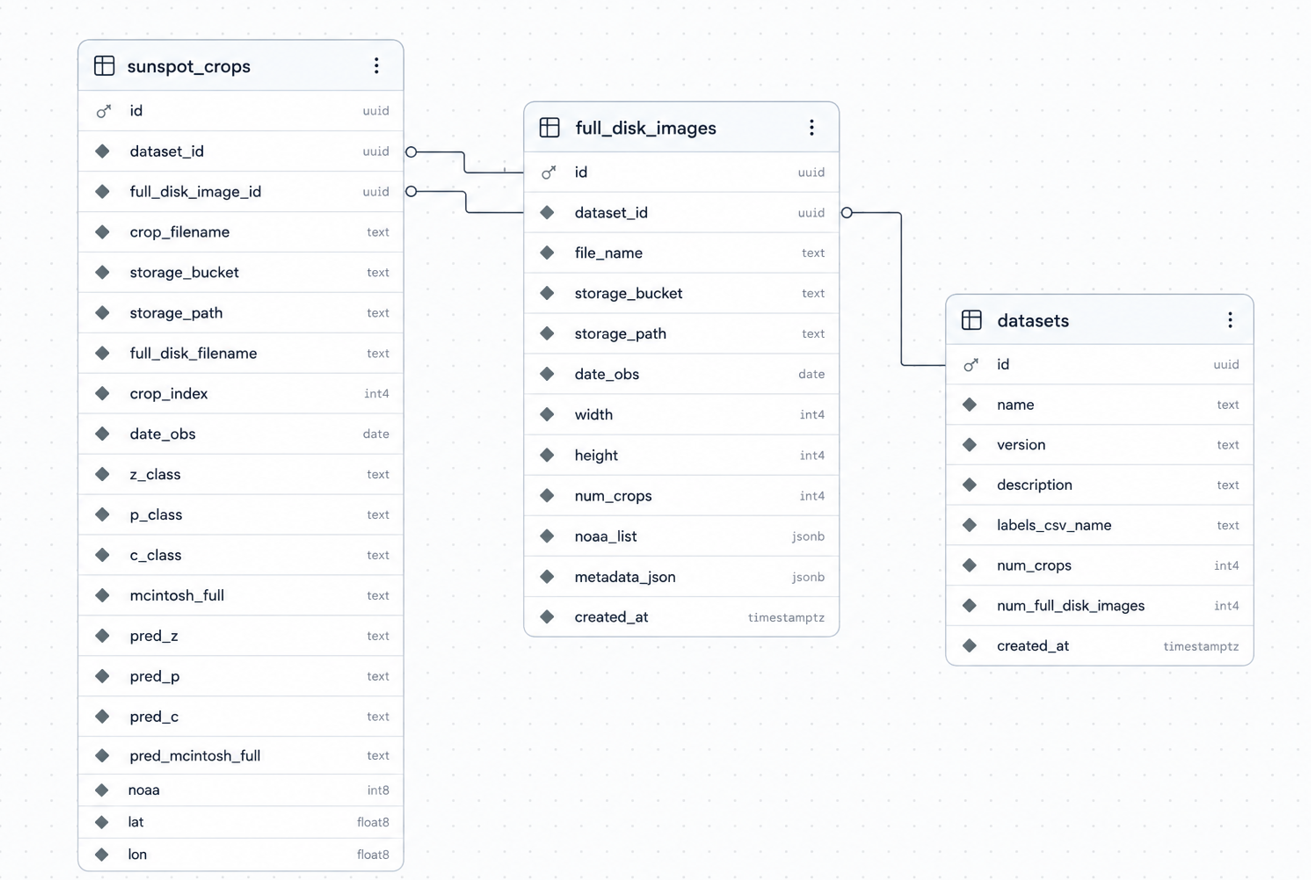
\includegraphics[width=0.92\textwidth]{figures/data/db_schema.png}
    \caption{Esquema lógico de datos para observaciones solares, regiones activas,
    recortes, etiquetas e inferencias. La separación entre entidades permite
    consultar resultados sin perder la relación con la imagen original y los
    metadatos NOAA/SRS. \textbf{Fuente:} Elaboración propia.}
    \label{fig:db-schema-data}
\end{figure}

La construcción de DB2 no consiste simplemente en recortar una vecindad fija
alrededor de cada coordenada NOAA. El procedimiento verifica la posición
proyectada sobre el disco, recorta una región suficientemente amplia para incluir
la estructura completa del grupo y luego reubica el recorte en un lienzo normalizado.
Así se evita deformar grupos alargados o regiones cercanas al limbo, donde la
proyección introduce cambios de escala aparente. La Figura~\ref{fig:hat-db2-pipeline-sw}
resume visualmente esta cadena de construcción.

\begin{figure}[H]
    \centering
    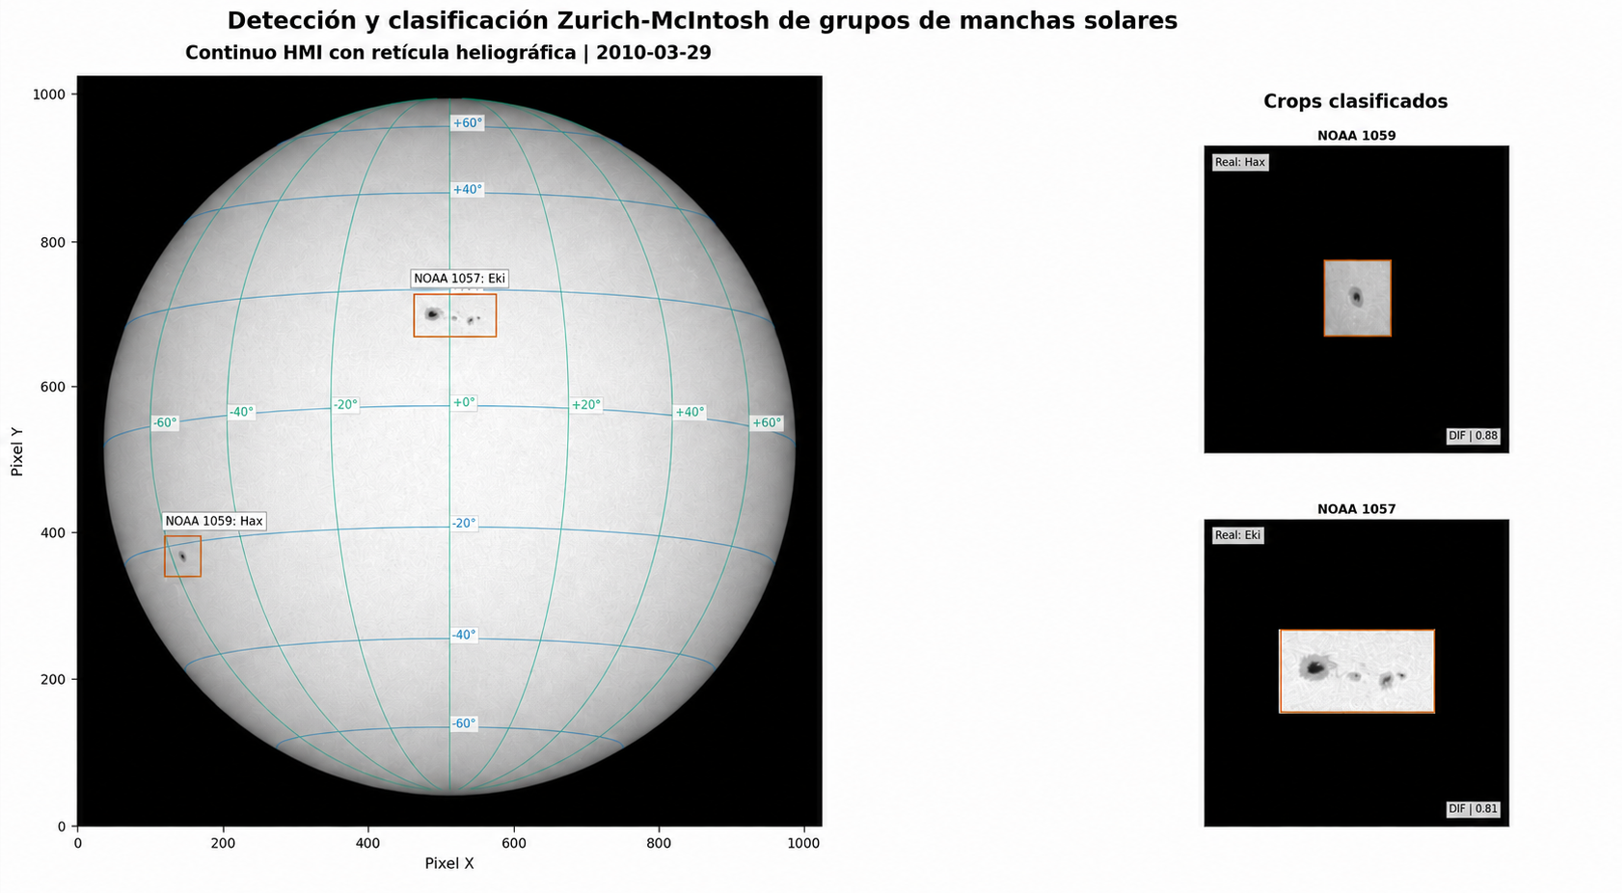
\includegraphics[width=\textwidth]{figures/data/db2_build.png}
    \caption{Construcción ilustrativa de DB2 a partir de una imagen
    SDO/HMI de disco completo con retícula heliográfica. La figura muestra la
    detección de grupos solares sobre el disco, su asociación con regiones NOAA y
    los recortes resultantes utilizados como ejemplos etiquetados para la
    clasificación Zurich--McIntosh. \textbf{Fuente:} Elaboración propia.}
    \label{fig:hat-db2-pipeline-sw}
\end{figure}

La Figura~\ref{fig:db2-zpc-sw} resume la frecuencia de las combinaciones
Zurich--McIntosh presentes en DB2. La distribución es desbalanceada: pocas
configuraciones concentran gran parte de los registros y muchas combinaciones
aparecen con baja frecuencia. Esta estructura condiciona el aprendizaje
supervisado y la interpretación de los errores.

\begin{figure}[H]
    \centering
    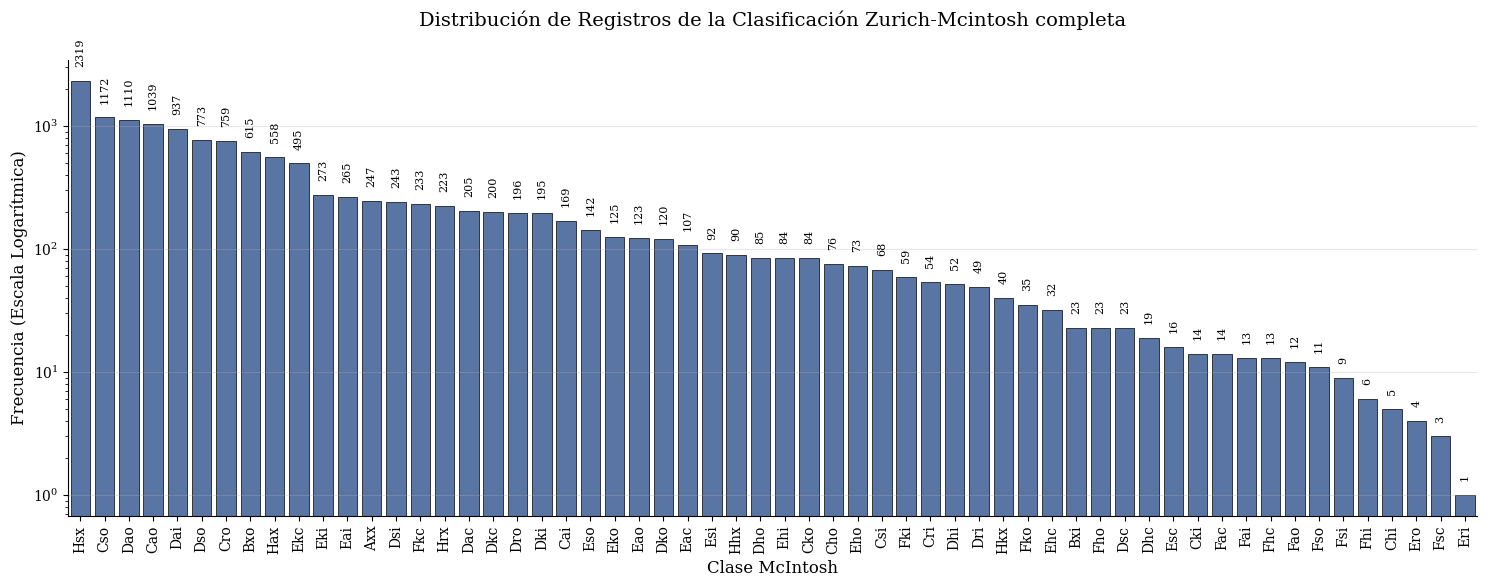
\includegraphics[width=\textwidth]{figures/data/class_hist.png}
    \caption{Histograma de frecuencias por combinación Zurich--McIntosh ($ZPC$)
    de DB2. Se aprecia un régimen de cola larga, donde unas pocas combinaciones
    dominan la muestra total. \textbf{Fuente:} Elaboración propia.}
    \label{fig:db2-zpc-sw}
\end{figure}

La Figura~\ref{fig:db2-caracteres-sw} desagrega la misma base por componente de
la taxonomía. Las distribuciones marginales de $Z$, $P$ y $C$ confirman que el
desbalance no se limita a la combinación completa, sino que afecta cada salida de
forma distinta. Por ello, el entrenamiento requiere ponderación, muestreo
balanceado y evaluación separada por componente.

\begin{figure}[H]
    \centering
    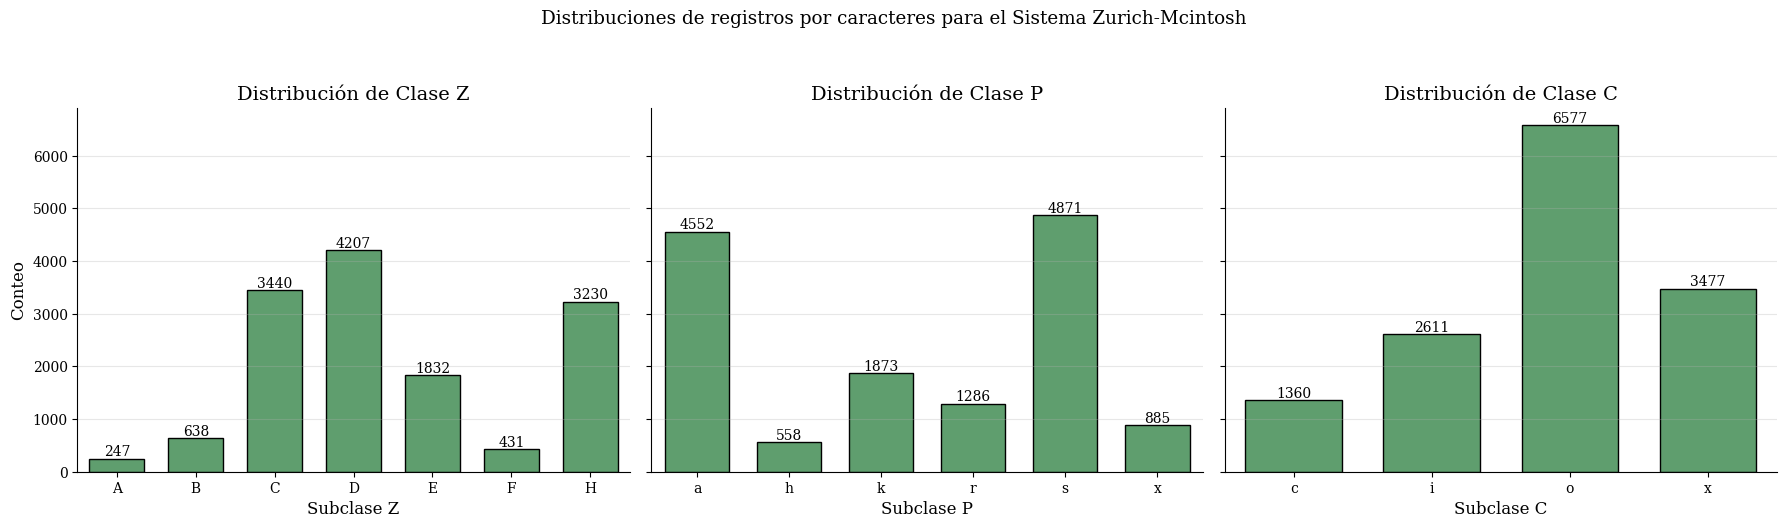
\includegraphics[width=\textwidth]{figures/data/char_hist.png}
    \caption{Histogramas de frecuencias por carácter en DB2 para las componentes
    $Z$, $P$ y $C$ de la clasificación Zurich--McIntosh. La desagregación
    evidencia la asimetría marginal de cada salida. \textbf{Fuente:} Elaboración propia.}
    \label{fig:db2-caracteres-sw}
\end{figure}

Además del desbalance, la generación automática de recortes introduce ruido
residual: regiones parciales, agrupamientos ambiguos o recortes con contaminación
geométrica. Para reducir estos casos se empleó una depuración basada en reducción
de dimensión con PCA y detección de valores atípicos mediante \textit{Isolation
Forest}. Esta etapa no elimina la ambigüedad propia del dominio, pero mejora la
coherencia morfológica del conjunto y favorece un entrenamiento más estable.

Con estas dos bases queda definido el insumo principal de la etapa de aprendizaje
profundo: DB1 permite enseñar al sistema dónde se encuentran los grupos solares
en el disco completo, mientras que DB2 permite enseñar qué morfología presenta
cada región activa una vez recortada. La arquitectura de IA se construye a partir
de esta división funcional.

\section{Entrenamiento de modelos de Deep Learning}
\label{sec:training}

La arquitectura de aprendizaje profundo se organiza como una cascada modular. En
la primera etapa, un detector localiza grupos de manchas solares en imágenes de
disco completo. En la segunda etapa, un clasificador especializado recibe los
recortes generados por el detector y estima las componentes de la taxonomía
Zurich--McIntosh. Esta separación reduce la complejidad de cada tarea: el detector
se concentra en ubicación espacial y el clasificador en morfología local.

El enfoque en cascada también mejora la trazabilidad del sistema. Cada predicción
puede asociarse con una región detectada, una fecha, una posición heliográfica y
una etiqueta taxonómica. En caso de error, es posible distinguir si la falla
proviene de la localización inicial, del recorte utilizado o de la clasificación
morfológica posterior.

\subsection{YOLO26n}

La etapa de agrupamiento se implementa con YOLO26n para localizar grupos de
manchas solares en imágenes de disco completo. El modelo se entrenó sobre DB1, compuesta por imágenes HMI de disco completo con
anotaciones de grupos solares. Antes del entrenamiento definitivo, las etiquetas
obtenidas por acoplamiento entre imágenes y registros observacionales fueron
revisadas en Roboflow, con el fin de corregir cajas desplazadas, regiones
omitidas y detecciones espurias. Esta revisión técnico-visual complementa el etiquetado
automático y mejora la coherencia espacial del conjunto de detección. Además, se
aplicó una aumentación de datos en Roboflow que expandió las 4700 imágenes
etiquetadas originales a 10958 imágenes, utilizando volteo horizontal
(\textit{Flip: Horizontal}) y rotaciones de 90° en sentido horario y antihorario
(\textit{90° Rotate: Clockwise, Counter-Clockwise}). Estas transformaciones
controladas incrementan la robustez frente a cambios de orientación y posición
aparente de las regiones sobre el disco.

\begin{figure}[H]
    \centering
    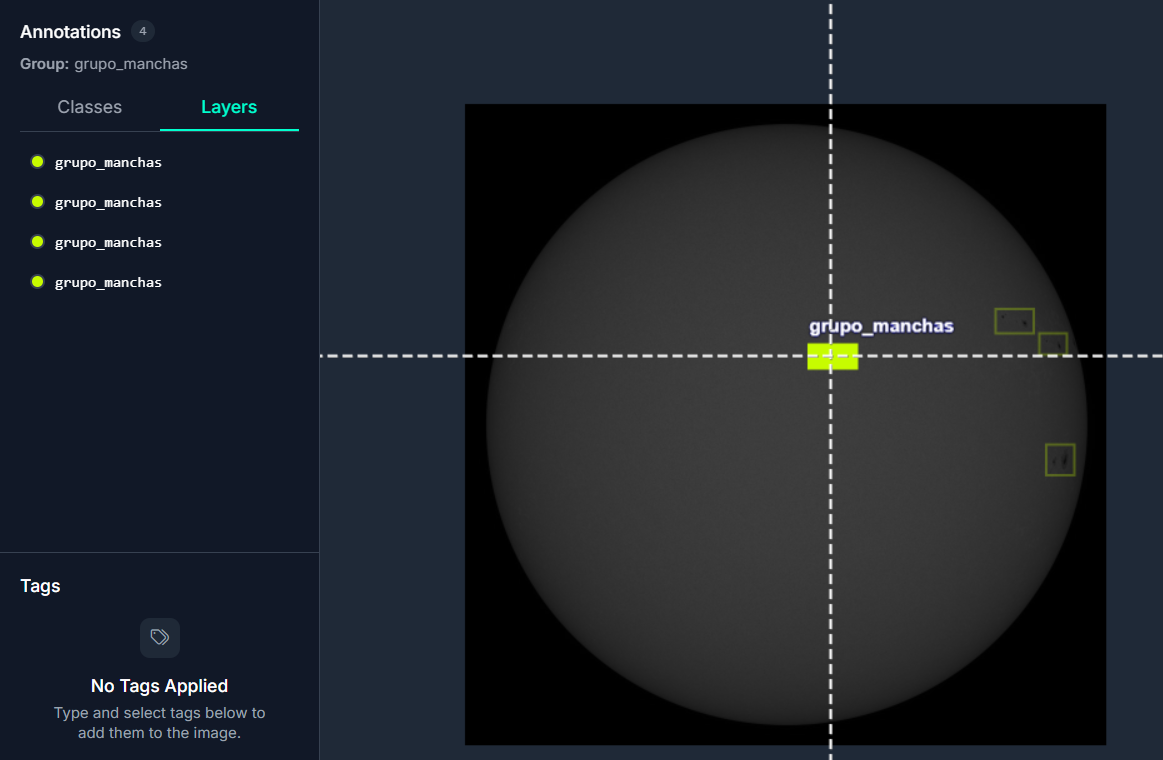
\includegraphics[width=0.92\textwidth]{figures/ml/roboflow.png}
    \caption{Configuración del conjunto de detección en Roboflow, incluyendo la
    revisión de anotaciones y las transformaciones de aumentación aplicadas a las
    imágenes etiquetadas. \textbf{Fuente:} Elaboración propia.}
    \label{fig:roboflow-yolo-augmentation}
\end{figure}

El entrenamiento se realizó durante 200 épocas con tamaño de entrada de 640
píxeles. La configuración final de hiperparámetros se obtuvo mediante Optuna,
explorando tasa de aprendizaje, tamaño de lote, regularización, aumentos de datos
y parámetros de optimización. La selección del modelo consideró métricas estándar
de detección, como precisión, \textit{recall}, intersección sobre unión (IoU) y
precisión media promedio (mAP), junto con la estabilidad de las curvas de pérdida
durante entrenamiento y validación.

Los resultados muestran una convergencia estable y un equilibrio adecuado entre
precisión y exhaustividad para la localización de grupos solares. Sin embargo,
debido a que el entrenamiento se basa en imágenes HMI acopladas con reportes NOAA
SRD, estas métricas deben interpretarse como una validación de la etapa de
localización dentro del dominio fotosférico de entrenamiento. La operación final
en imágenes luz blanca puede requerir ajustes adicionales para compensar
diferencias de contraste, resolución efectiva, \textit{seeing} y condiciones de
adquisición terrestre.

Para el despliegue, el detector se exporta al formato ONNX (\textit{Open Neural
Network Exchange}), en coherencia con la estrategia general de inferencia del
sistema. Esta conversión permite ejecutar el modelo mediante motores compatibles
con entornos locales y web, reduciendo la dependencia del entorno original de
entrenamiento. La portabilidad del detector es especialmente relevante porque la
calidad de sus cajas condiciona las etapas posteriores de recorte, clasificación
y trazabilidad observacional.

La Figura~\ref{fig:yolo-training-results} resume las métricas de entrenamiento
del detector YOLO26n sobre DB1. Las curvas muestran la evolución de las pérdidas
y de los indicadores de precisión, \textit{recall} y mAP, permitiendo verificar
que el modelo alcanza un punto de operación adecuado para construir y refinar
DB2.

\begin{figure}[H]
    \centering
    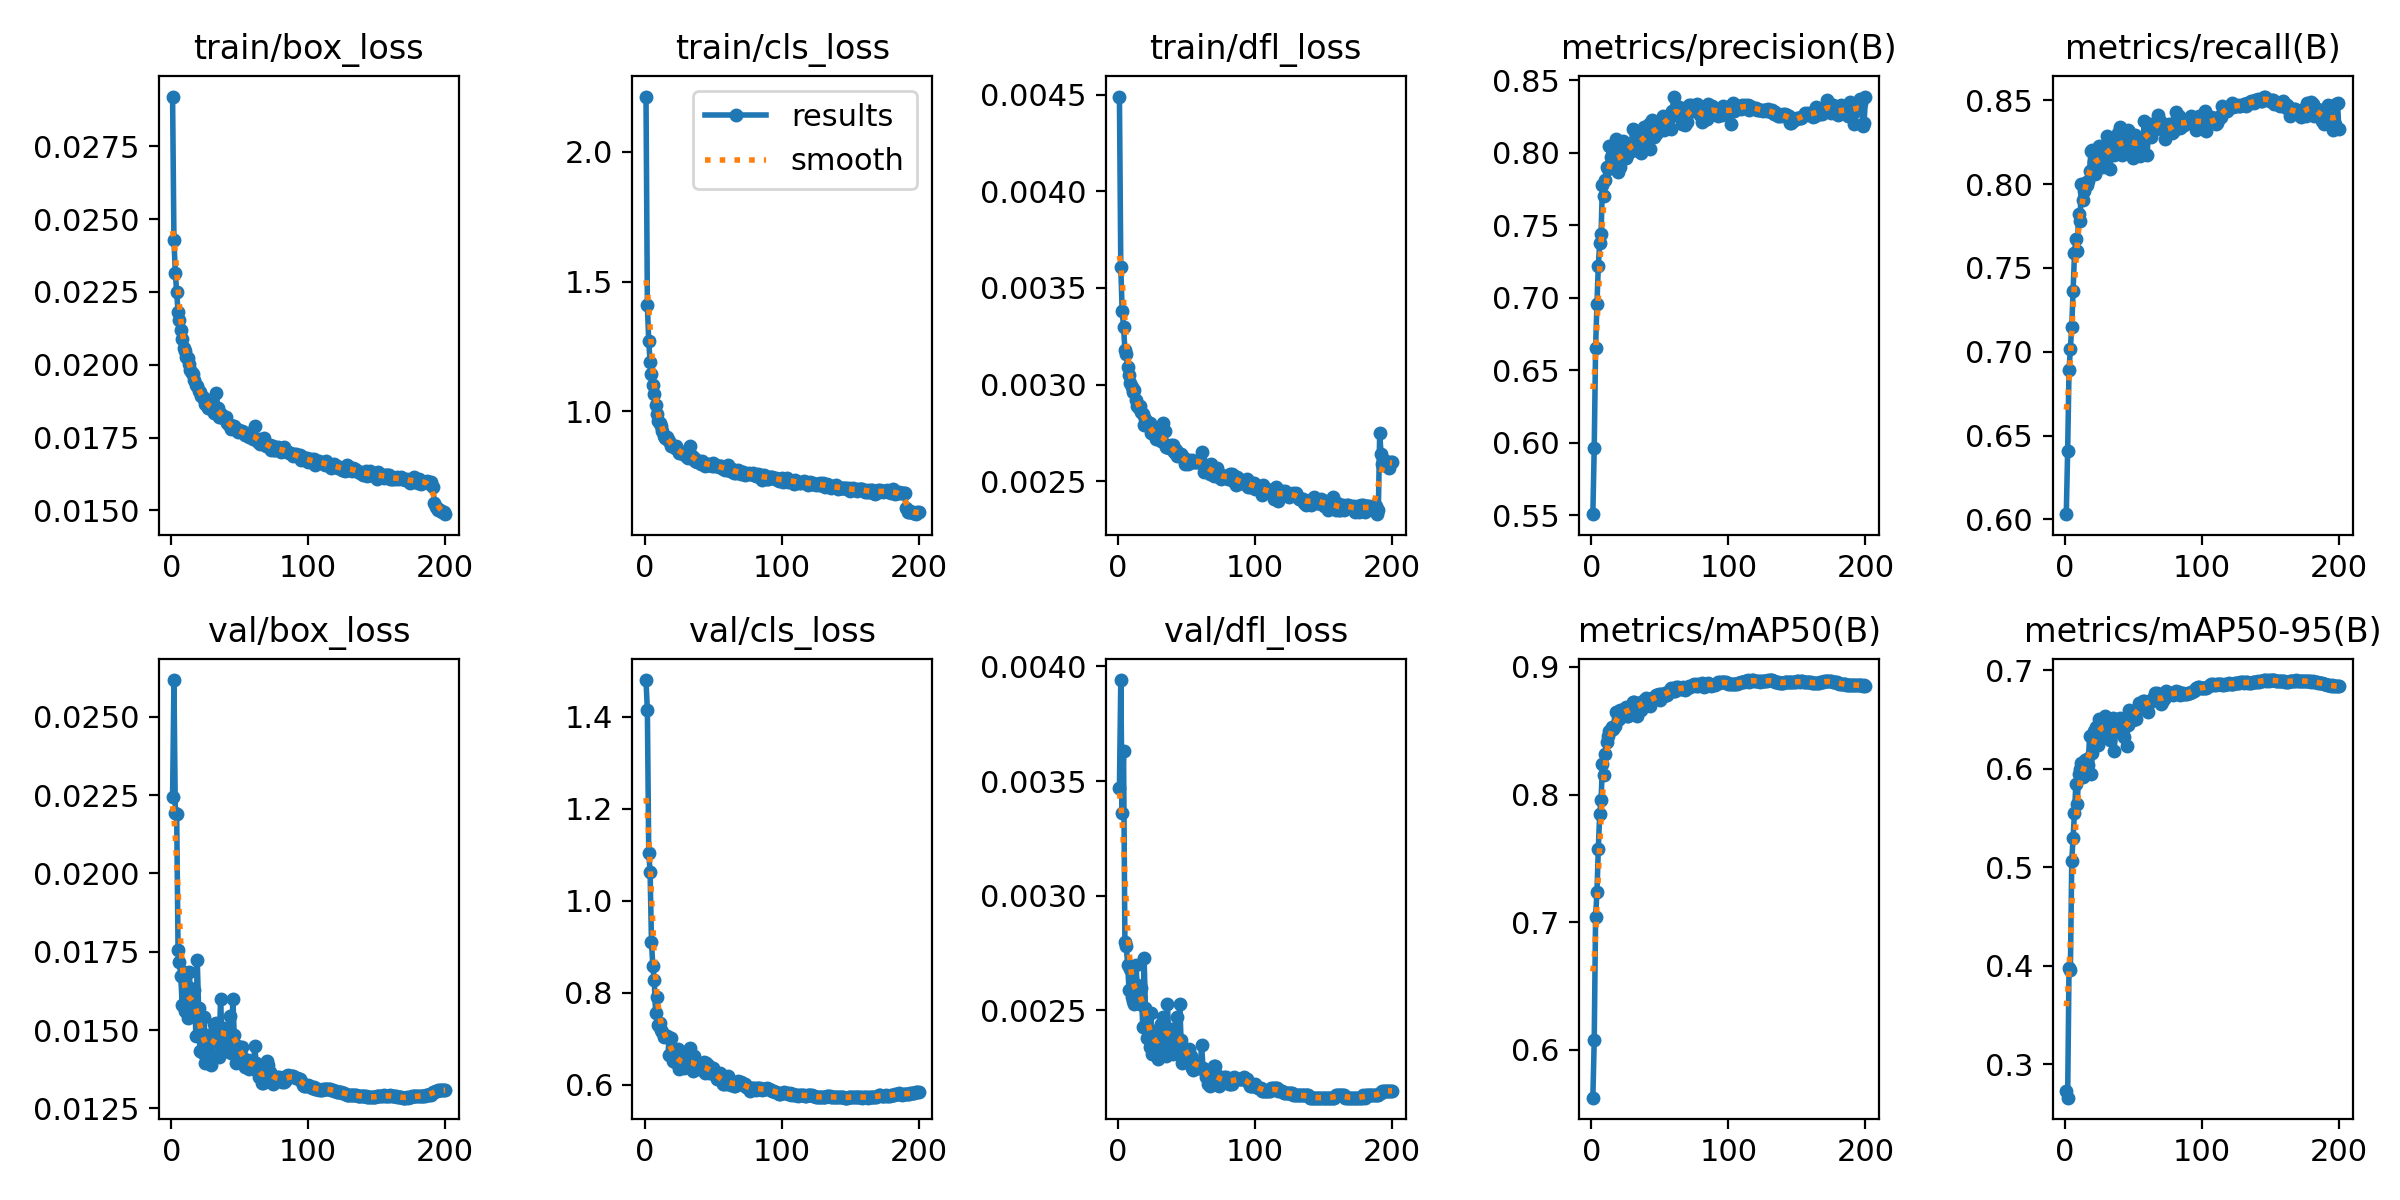
\includegraphics[width=0.92\textwidth]{figures/ml/yolo_results.png}
    \caption{Métricas de entrenamiento del detector YOLO26n sobre DB1. Se
    muestran la evolución de las pérdidas de entrenamiento y validación, junto
    con las métricas de precisión, \textit{recall} y mAP utilizadas para evaluar
    la convergencia del modelo durante el aprendizaje. \textbf{Fuente:} Elaboración propia.}
    \label{fig:yolo-training-results}
\end{figure}

\subsection{ConvNeXtV2}

La etapa de clasificación utiliza ConvNeXtV2 Atto como extractor visual profundo para
inferir las componentes $Z$, $P$ y $C$ de la taxonomía Zurich--McIntosh. El
modelo se inicializa con pesos preentrenados sobre ImageNet y posteriormente se
ajusta finamente sobre la base DB2.1, lo que permite reutilizar representaciones
visuales generales y adaptarlas a rasgos morfológicos característicos de manchas
solares \citep{deng2009imagenet,woo2023convnextv2,zhou2023mcintosh}.

\begin{figure}[H]
    \centering
    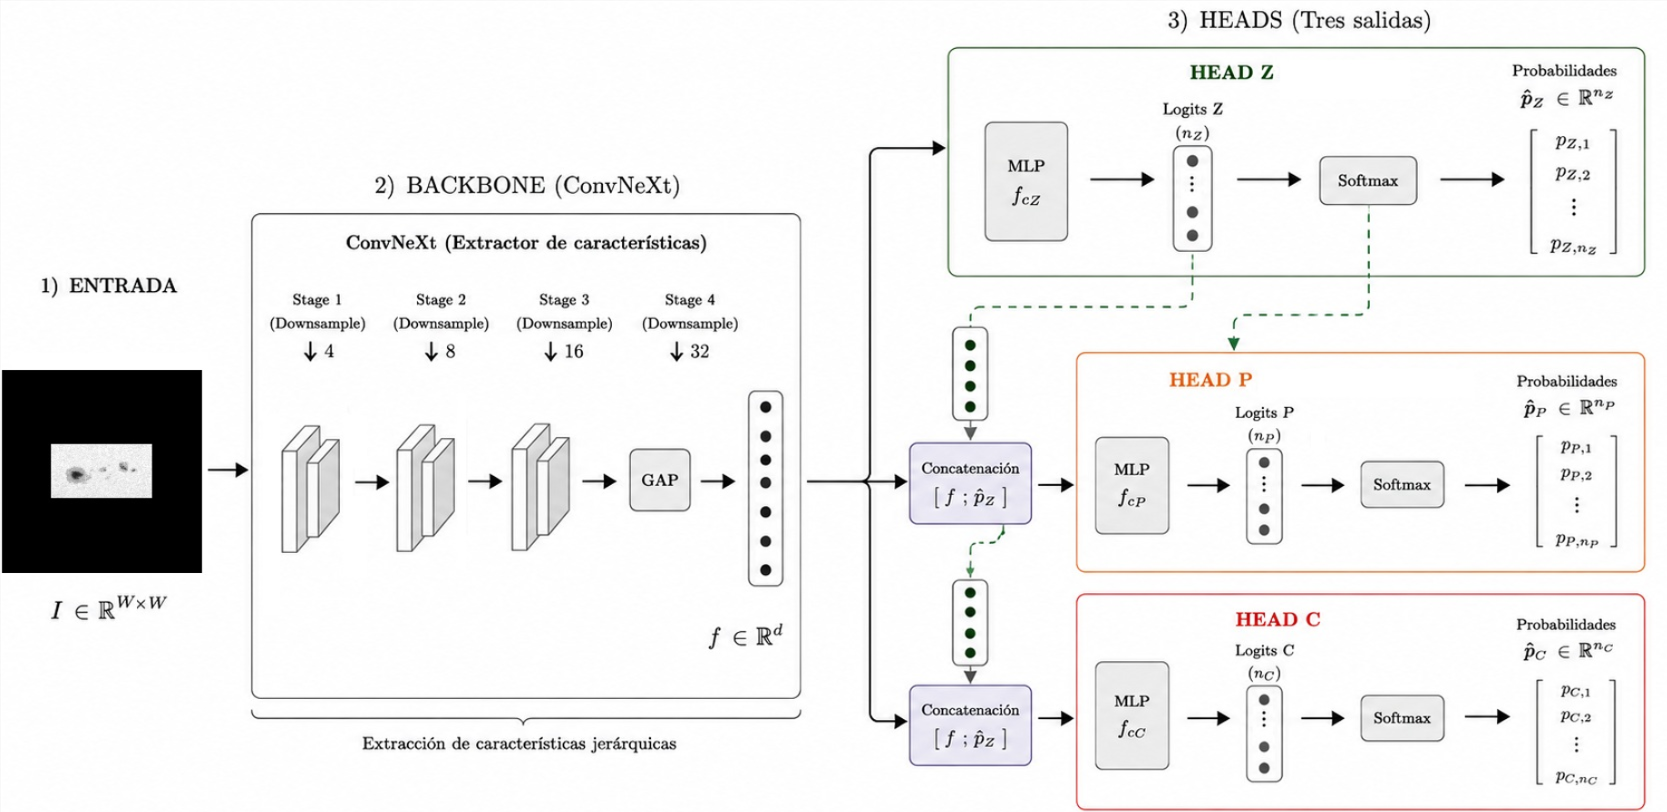
\includegraphics[width=\textwidth]{figures/ml/convnext_arch.png}
    \caption{Arquitectura jerárquica del clasificador ConvNeXtV2 Atto propuesto para
    la inferencia de la taxonomía Zurich--McIntosh. El modelo
    extrae un vector global de características mediante el backbone ConvNeXtV2 y
    genera primero la distribución probabilística del carácter Zurich ($Z$). El
    vector global se obtiene mediante agrupamiento promedio global (GAP), y las
    distribuciones de las componentes $P$ y $C$ se calculan a partir de la
    concatenación $[\mathbf{f};\hat{\mathbf{p}}_Z]$, preservando la estructura
    jerárquica de la taxonomía. \textbf{Fuente:} Elaboración propia.}
    \label{fig:convnextv2-hierarchical}
\end{figure}

La Figura~\ref{fig:convnextv2-hierarchical} resume la arquitectura jerárquica
adoptada. El clasificador recibe recortes de regiones activas insertados en una
matriz de $224 \times 224$ píxeles, preservando la proporción del recorte para
evitar distorsiones por redimensionamiento. Estos recortes provienen de la etapa
YOLO26n y constituyen la entrada del modelo ConvNeXtV2.

El backbone ConvNeXtV2 Atto transforma cada recorte mediante una secuencia de
\textit{stages} jerárquicos con reducciones progresivas de resolución espacial.
Durante el ajuste fino, estos \textit{stages} se incorporan de manera progresiva
al entrenamiento, permitiendo que las capas finales se adapten primero al dominio
solar y que los bloques profundos se actualicen después con menor riesgo de
perder las representaciones generales aprendidas durante el preentrenamiento.
Al final del extractor, una operación de agrupamiento promedio global (GAP,
\textit{Global Average Pooling}) resume los mapas de características en un vector
latente global
\[
\mathbf{f} \in \mathbb{R}^{d},
\]
que concentra información de contraste, textura, geometría y organización del
grupo solar. A partir de esta representación se calcula primero la distribución
del carácter Zurich,
\[
\hat{\mathbf{p}}_Z \in \mathbb{R}^{n_Z},
\]
mediante una salida MLP seguida de Softmax. Las salidas de $P$ y $C$ reciben la
concatenación $[\mathbf{f};\hat{\mathbf{p}}_Z]$, incorporando la dependencia
jerárquica de la taxonomía, y producen
\[
\hat{\mathbf{p}}_P \in \mathbb{R}^{n_P},
\qquad
\hat{\mathbf{p}}_C \in \mathbb{R}^{n_C}.
\]
Por tanto, la salida del modelo se expresa como
\[
f_\theta(x)=
\left(
\hat{\mathbf{p}}_Z,
\hat{\mathbf{p}}_P,
\hat{\mathbf{p}}_C
\right),
\]
donde cada término es una distribución de probabilidad sobre una componente
taxonómica.

Esta descomposición evita tratar cada combinación Zurich--McIntosh como una
clase atómica. Aunque el espacio completo contiene alrededor de 60
configuraciones válidas, el aprendizaje directo sobre combinaciones completas
incrementaría el desbalance y limitaría la generalización en clases raras. La
Figura~\ref{fig:db2-train-val-caracter} muestra que la partición de
entrenamiento y validación conserva la asimetría de DB2 en las tres salidas.

\begin{figure}[H]
    \centering
    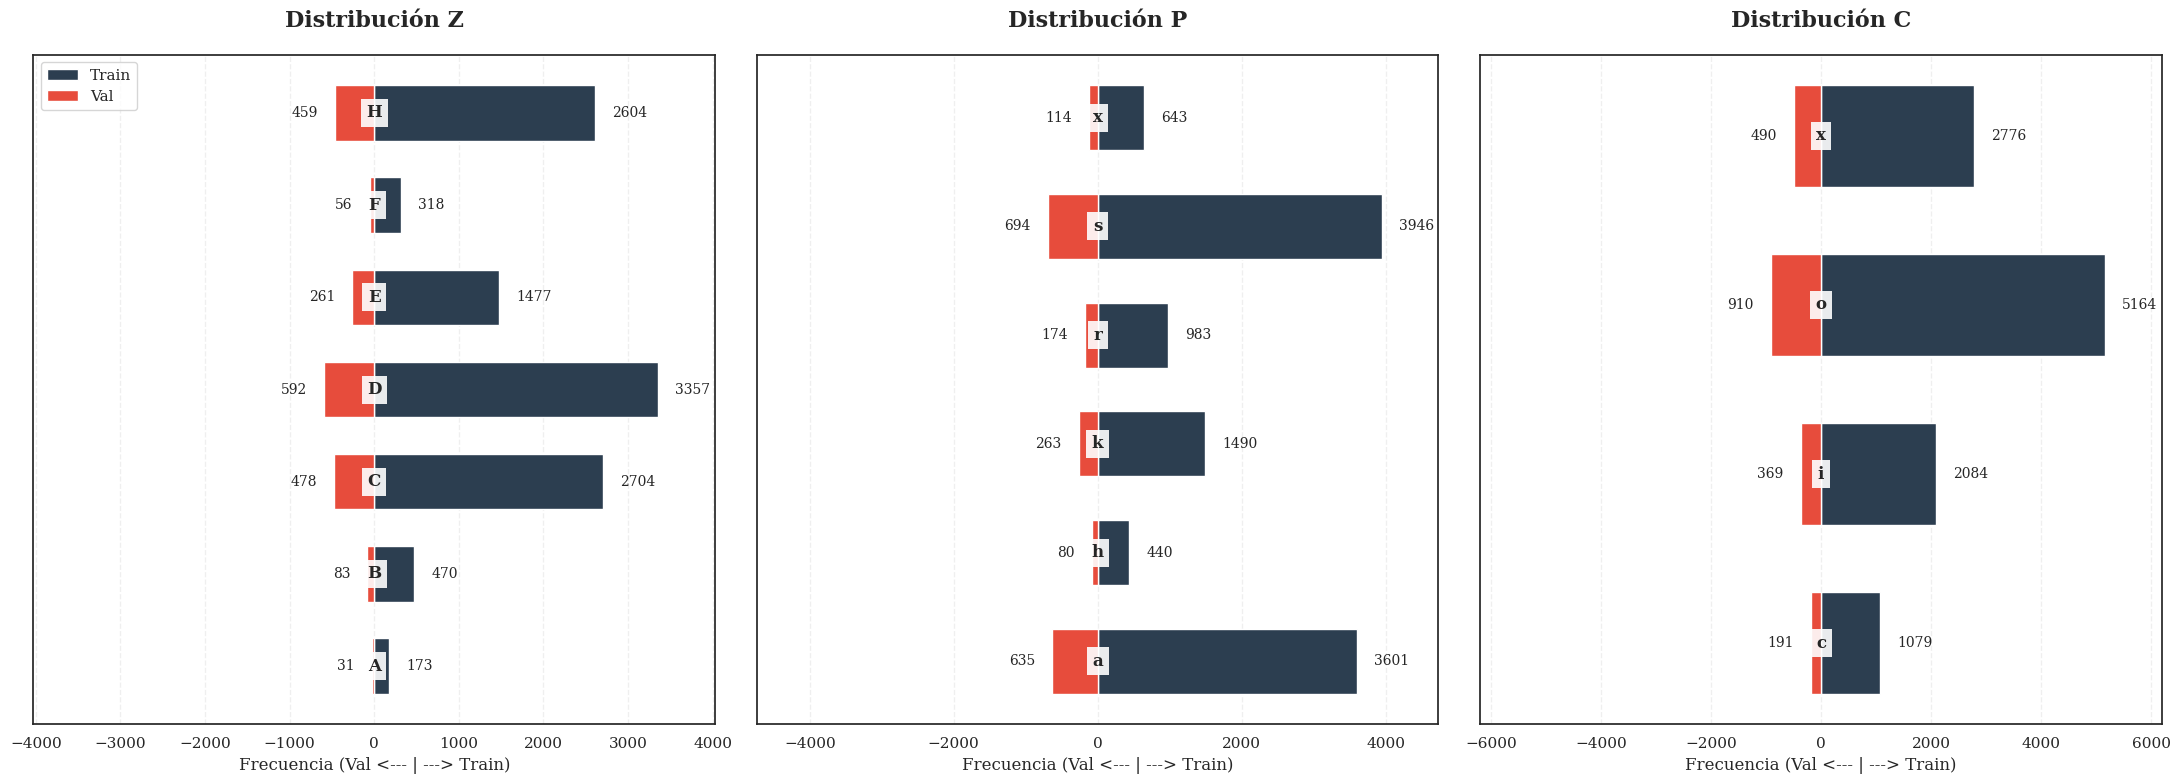
\includegraphics[width=\textwidth]{figures/data/train_val.png}
    \caption{Distribución de frecuencias en los subconjuntos de entrenamiento y
    validación para las componentes $Z$, $P$ y $C$ de la clasificación
    Zurich--McIntosh sobre DB2. La figura muestra que el desbalance de clases se
    mantiene en ambas particiones, con distinta severidad según el carácter
    considerado. \textbf{Fuente:} Elaboración propia.}
    \label{fig:db2-train-val-caracter}
\end{figure}

El entrenamiento mitiga el desbalance mediante pesos basados en el número
efectivo de muestras, muestreo balanceado con \textit{WeightedRandomSampler} y
seguimiento separado de métricas para $Z$, $P$ y $C$ \citep{cui2019classbalanced}.
La arquitectura emplea
Optuna para determinar una configuración óptima de hiperparámetros de
entrenamiento, explorando tasa de aprendizaje, \textit{weight decay}, tamaño de
lote, aumentos, configuración de las salidas MLP y estrategia de ajuste
progresivo de los \textit{stages}. La selección final considera desempeño en
validación, estabilidad de entrenamiento y consistencia entre salidas, no solo la
exactitud global \citep{akiba2019optuna}.

El monitoreo se realiza con curvas de pérdida, exactitud por salida y análisis de
generalización. En los experimentos se observó sobreajuste antes de completar el
máximo de épocas programado, por lo que se conserva el punto con mejor desempeño
en validación. Las Figuras~\ref{fig:cm-z}, \ref{fig:cm-p} y \ref{fig:cm-c}
presentan las matrices de confusión normalizadas: $C$ muestra una separación más
estable, mientras que $Z$ y $P$ concentran ambigüedad en clases fronterizas o con
menor soporte muestral.

Antes de presentar las tablas por clase y las matrices de confusión, se definen
las métricas empleadas para evaluar cada salida del clasificador. Para una clase
$c$ de cualquiera de las salidas $Z$, $P$ o $C$, sean $TP_c$ los verdaderos
positivos, $FP_c$ los falsos positivos y $FN_c$ los falsos negativos. La
precisión de la clase se calcula como
\begin{equation}
\mathrm{Precision}_c=\frac{TP_c}{TP_c+FP_c}.
\end{equation}

El \textit{recall}, o sensibilidad, mide la proporción de ejemplos de la clase
$c$ correctamente recuperados por el modelo:
\begin{equation}
\mathrm{Recall}_c=\frac{TP_c}{TP_c+FN_c}.
\end{equation}

A partir de ambas cantidades, el puntaje F1 se define como la media armónica
entre precisión y \textit{recall}:
\begin{equation}
\mathrm{F1}_c=2\,\frac{\mathrm{Precision}_c\,\mathrm{Recall}_c}{\mathrm{Precision}_c+\mathrm{Recall}_c}.
\end{equation}

En las tablas siguientes se reportan estas métricas por clase y su promedio
ponderado. Este último considera el soporte de cada clase en el conjunto de
validación, por lo que resulta más representativo en presencia de desbalance,
aunque debe interpretarse junto con las métricas individuales para identificar
clases minoritarias o morfológicamente ambiguas.


\begin{table}[H]
\centering
\caption{Resumen de métricas por clase para la salida $Z$. \textbf{Fuente:} Elaboración propia.}
\small
\setlength{\tabcolsep}{8pt}
\renewcommand{\arraystretch}{0.92}
\begin{tabular}{lccc}
\hline
\textbf{Clase} & \textbf{Precisión} & \textbf{Recall} & \textbf{F1} \\ \hline
A & 0.79 & 0.73 & 0.76 \\
B & 0.74 & 0.71 & 0.72 \\
C & 0.68 & 0.61 & 0.64 \\
D & 0.63 & 0.61 & 0.62 \\
E & 0.49 & 0.39 & 0.43 \\
F & 0.47 & 0.39 & 0.43 \\
H & 0.78 & 0.84 & 0.81 \\ \hline
Prom. pond. & 0.68 & 0.63 & 0.65 \\ \hline
\end{tabular}
\end{table}

\begin{figure}[H]
    \centering
    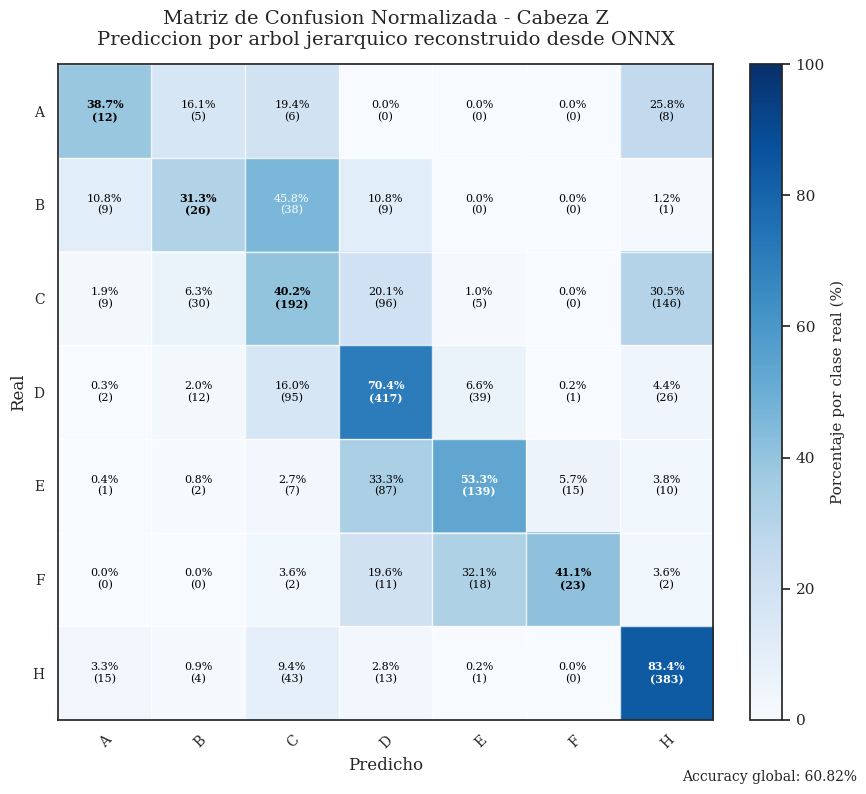
\includegraphics[width=0.75\textwidth]{figures/ml/conf_z.png}
    \caption{Matriz de confusión normalizada para la salida $Z$ del clasificador
    ConvNeXtV2. La diagonal dominante refleja aciertos en varias clases
    principales, mientras que las mayores confusiones se concentran entre
    categorías morfológicamente cercanas. \textbf{Fuente:} Elaboración propia.}
    \label{fig:cm-z}
\end{figure}

\begin{table}[H]
\centering
\caption{Resumen de métricas por clase para la salida $P$. \textbf{Fuente:} Elaboración propia.}
\small
\setlength{\tabcolsep}{8pt}
\renewcommand{\arraystretch}{0.92}
\begin{tabular}{lccc}
\hline
\textbf{Clase} & \textbf{Precisión} & \textbf{Recall} & \textbf{F1} \\ \hline
x & 0.57 & 0.31 & 0.40 \\
r & 0.34 & 0.28 & 0.31 \\
s & 0.59 & 0.63 & 0.61 \\
a & 0.46 & 0.54 & 0.50 \\
h & 0.71 & 0.65 & 0.68 \\
k & 0.84 & 0.82 & 0.83 \\ \hline
Prom. pond. & 0.66 & 0.61 & 0.63 \\ \hline
\end{tabular}
\end{table}

\begin{figure}[H]
    \centering
    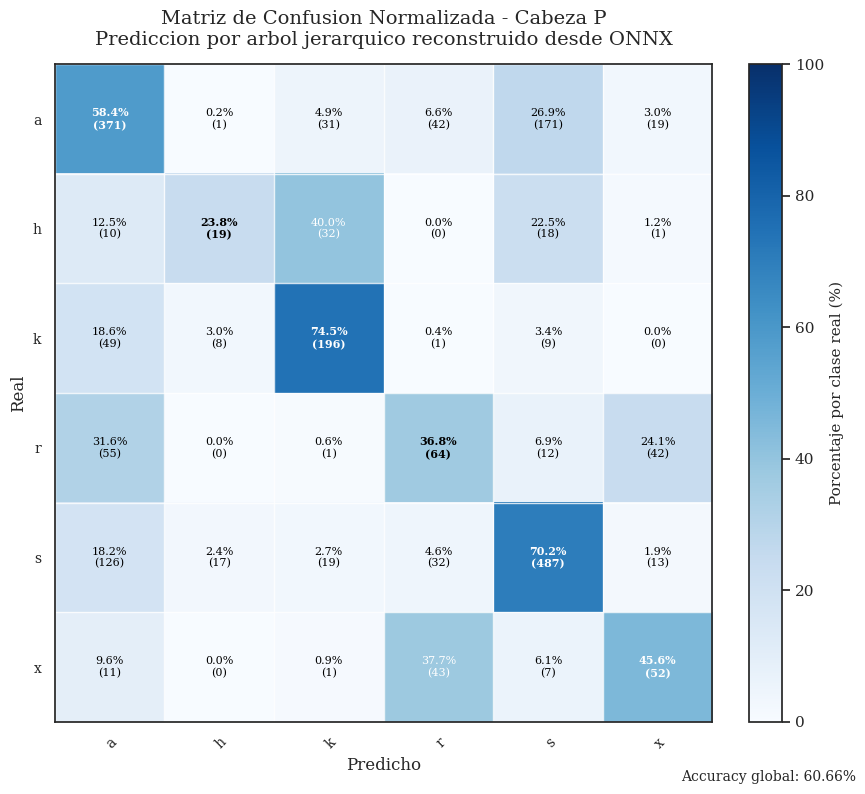
\includegraphics[width=0.75\textwidth]{figures/ml/conf_p.png}
    \caption{Matriz de confusión normalizada para la salida $P$ del modelo
    ConvNeXtV2. Parte importante del error se distribuye entre configuraciones
    penumbrales vecinas, en especial en clases con fuerte desbalance o menor
    número de ejemplos. \textbf{Fuente:} Elaboración propia.}
    \label{fig:cm-p}
\end{figure}

\begin{table}[H]
\centering
\caption{Resumen de métricas por clase para la salida $C$. \textbf{Fuente:} Elaboración propia.}
\small
\setlength{\tabcolsep}{8pt}
\renewcommand{\arraystretch}{0.92}
\begin{tabular}{lccc}
\hline
\textbf{Clase} & \textbf{Precisión} & \textbf{Recall} & \textbf{F1} \\ \hline
x & 0.62 & 0.52 & 0.57 \\
o & 0.46 & 0.47 & 0.46 \\
i & 0.79 & 0.72 & 0.75 \\
c & 0.82 & 0.84 & 0.83 \\ \hline
Prom. pond. & 0.74 & 0.69 & 0.71 \\ \hline
\end{tabular}
\end{table}

\begin{figure}[H]
    \centering
    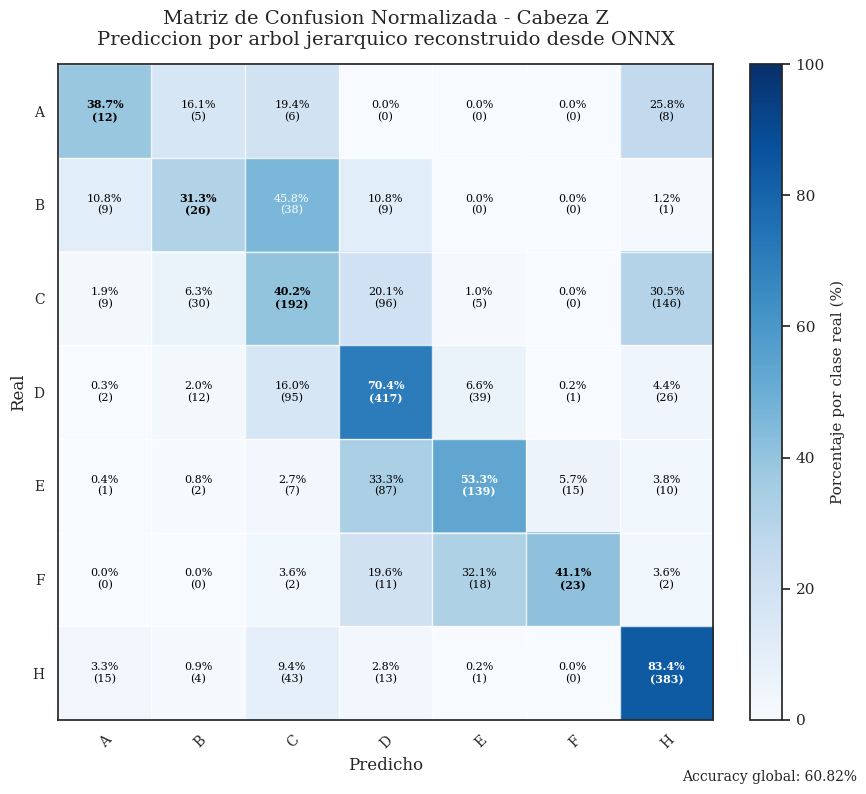
\includegraphics[width=0.75\textwidth]{figures/ml/conf_c.png}
    \caption{Matriz de confusión normalizada para la salida $C$ del clasificador
    ConvNeXtV2. La componente de compactación presenta una estructura de error
    más concentrada sobre la diagonal, lo que sugiere una discriminación
    relativamente más estable que en las otras dos salidas. \textbf{Fuente:} Elaboración propia.}
    \label{fig:cm-c}
\end{figure}

\section{Modelos predictivos}

Los modelos predictivos se presentan como la implementación computacional de la
formulación temporal y espacio-temporal desarrollada en los capítulos anteriores.
A diferencia de detección y clasificación, orientada a interpretar
regiones activas individuales, esta etapa utiliza los datos recopilados en DB1
como base histórica para reconstruir tendencias globales de actividad solar y su
distribución latitudinal, siguiendo la formulación metodológica presentada en la
Sección~\ref{sec:forecast}.

En este contexto, DB1 aporta la secuencia de observaciones de disco completo y
las regiones activas asociadas, permitiendo derivar series temporales del número
de manchas solares y representaciones discretizadas de la actividad por latitud.
Se consideran dos aproximaciones complementarias: un modelo escalar basado en la
trayectoria del número de manchas solares y un modelo espacio-temporal que
reconstruye la distribución latitudinal de la actividad. En ambos casos se evalúa
primero el ajuste de los modelos sobre la dinámica histórica observada y luego se
extiende la predicción hasta el cierre del ciclo solar 25, correspondiente a
finales de 2030. El objetivo no es producir una predicción operacional
definitiva, sino implementar las herramientas formuladas previamente para aportar
contexto temporal y contrastar tendencias con observaciones futuras.

\subsection{Modelo PVL con filtro de Kalman adaptativo}

El modelo PVL con filtro de Kalman adaptativo se utiliza para suavizar y proyectar
la serie temporal del número de manchas solares. La formulación representa la
actividad mediante un estado latente que evoluciona en el tiempo y se actualiza
con observaciones disponibles. La ganancia adaptativa permite ajustar el peso
relativo entre predicción y medición, lo que resulta útil ante ruido observacional
y cambios graduales en la dinámica del ciclo solar
\citep{kalman1960newapproach,podladchikova2012kalman}.

La salida se expresa como $\mathrm{SSN}_{\mathrm{PVLK}}$, una trayectoria escalar
que resume la evolución estimada del índice. Esta aproximación es compacta y
adecuada para describir tendencias globales, aunque no contiene información
espacial sobre la ubicación latitudinal de las regiones activas.

\begin{figure}[H]
    \centering
    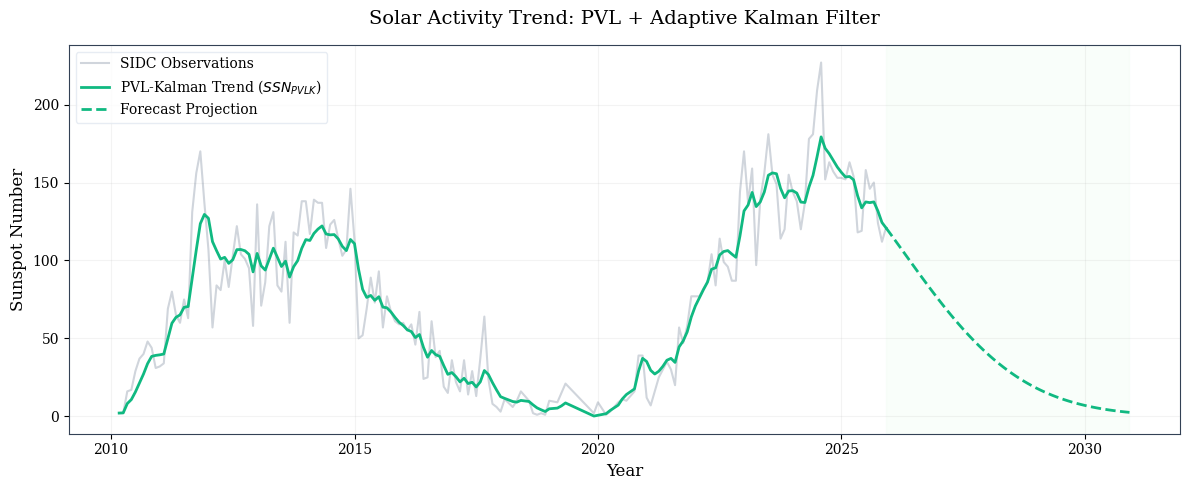
\includegraphics[width=0.92\textwidth]{figures/pred/kalman.png}
    \caption{Ajuste y predicción del número de manchas solares suavizado mediante
    el filtro de Kalman adaptativo ($\mathrm{SSN}_{\mathrm{PVLK}}$). Las líneas
    punteadas corresponden a la predicción. \textbf{Fuente:} Elaboración propia.}
    \label{fig:ssn-kalman-projection}
\end{figure}

\subsection{Modelo espacio-temporal del diagrama de Spörer con DMD}

El segundo enfoque utiliza la Descomposición en Modos Dinámicos (DMD) sobre una
representación latitudinal discretizada de la actividad solar. En lugar de modelar
solo una serie escalar, la actividad se organiza en una malla de latitudes donde
cada celda resume la presencia o intensidad relativa de regiones activas. Esta
representación permite aproximar la evolución espacio-temporal de las bandas de
actividad durante el ciclo solar \citep{schmid2010dmd,kutz2016dmd}.

DMD estima un operador lineal efectivo $\mathbf{A}$ que relaciona estados
consecutivos de la distribución latitudinal. Aunque la dinámica solar real no es
lineal, esta aproximación ofrece una descripción compacta de patrones dominantes
y permite reconstruir la migración progresiva de actividad hacia el ecuador,
rasgo característico del diagrama de Spörer. En términos teóricos, DMD puede
entenderse como una aproximación finita de modos dominantes asociados al operador
de Koopman; por ello puede capturar estructuras lineales efectivas de un sistema
subyacente no lineal cuando la dinámica observada está dominada por patrones
coherentes \citep{kutz2016dmd}.

\subsubsection{Diagrama de mariposa obtenido}

El diagrama de mariposa obtenido resume la evolución latitudinal de la actividad
reconstruida. Esta visualización permite evaluar si el modelo conserva una estructura
físicamente coherente, más allá de su error escalar sobre el número total de
manchas.

\begin{figure}[H]
    \centering
    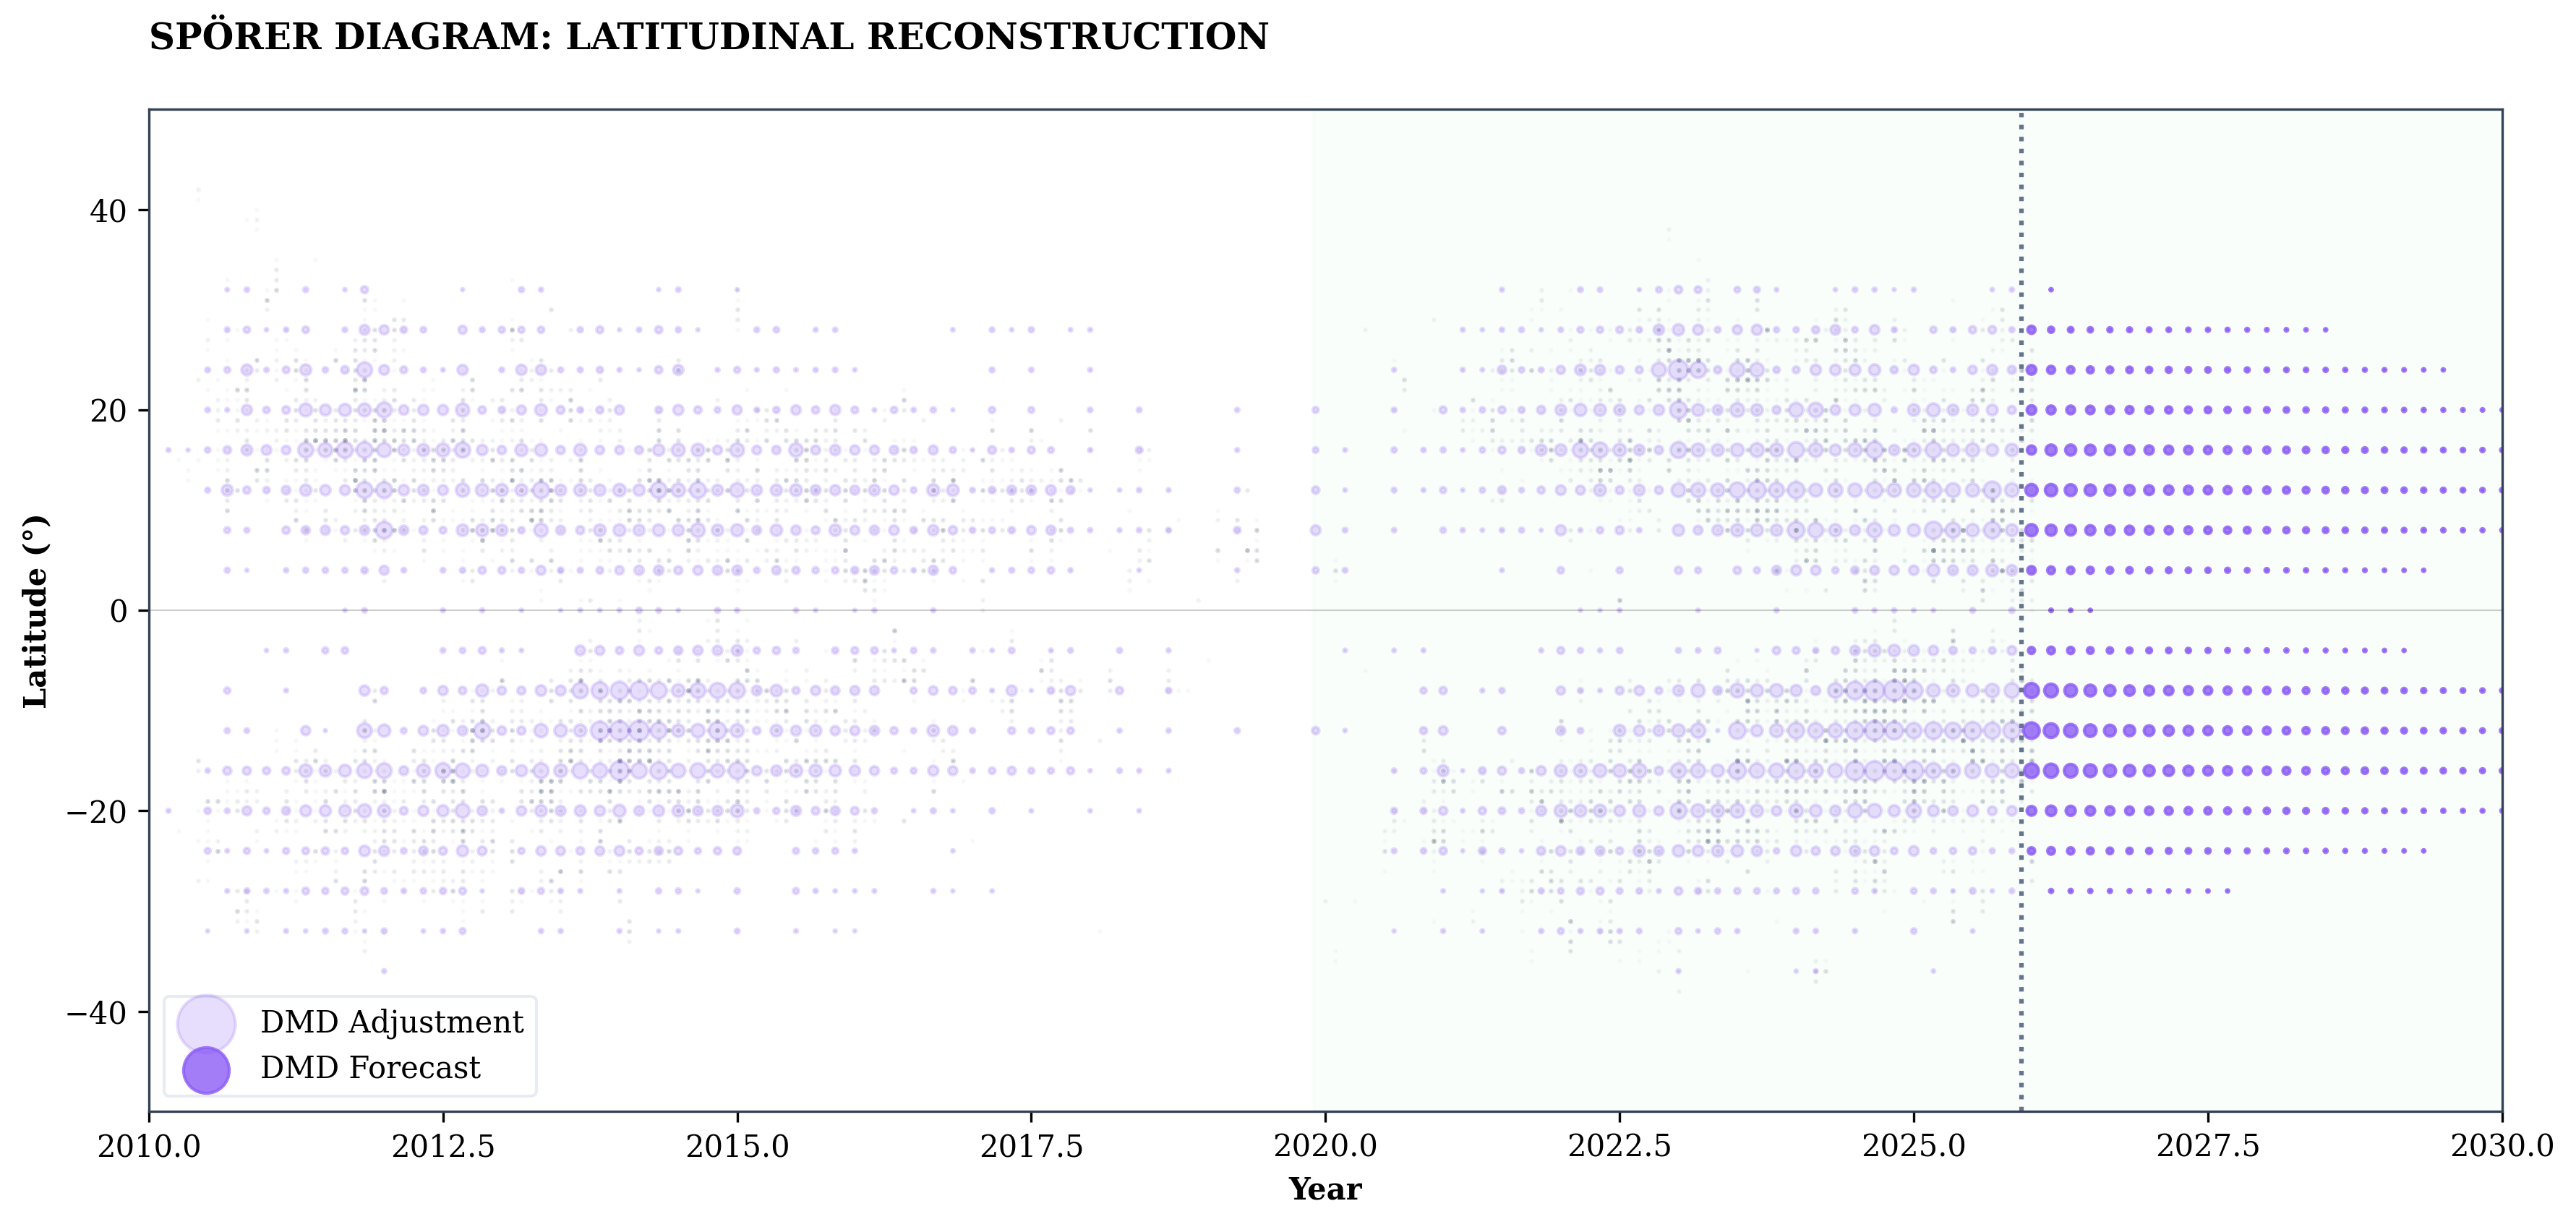
\includegraphics[width=0.92\textwidth]{figures/pred/sporer.png}
    \caption[Ajuste y predicción de la migración latitudinal con DMD]{Ajuste y predicción de la migración latitudinal de la actividad
    solar reconstruida mediante DMD. La figura ilustra el desplazamiento
    progresivo de las bandas activas hacia el ecuador (diagrama de Spörer)
    derivado del operador dinámico $\mathbf{A}$. La región con morado más intenso
    corresponde a la predicción. \textbf{Fuente:} Elaboración propia.}
    \label{fig:sporer-migration-model}
\end{figure}

\subsubsection{Cálculo del SSN por integral discreta}

Para comparar el modelo DMD con una serie escalar, la distribución latitudinal
reconstruida se reduce mediante una integral discreta sobre las celdas de la
malla. Manteniendo la misma formulación de la Sección~\ref{sec:forecast}, si
$\widehat{V}_j(t)$ representa la actividad estimada en la celda latitudinal $j$
para el instante $t$, el índice reconstruido se expresa como
\begin{equation}
\mathrm{SSN}_{\mathrm{DMD}}(t)=\kappa\sum_{j=1}^{M}\widehat{V}_j(t),
\end{equation}
donde $\kappa$ calibra la suma latitudinal respecto a la escala histórica:
\begin{equation}
\kappa=\frac{\sum_{t=1}^{N}\mathrm{SSN}_{\mathrm{obs}}(t)}{\sum_{t=1}^{N}\sum_{j=1}^{M}\widehat{V}_j(t)}.
\end{equation}
Esta operación no reemplaza la interpretación espacial del modelo; solo permite
obtener una magnitud comparable con el número de manchas solares tradicional.

\begin{figure}[H]
    \centering
    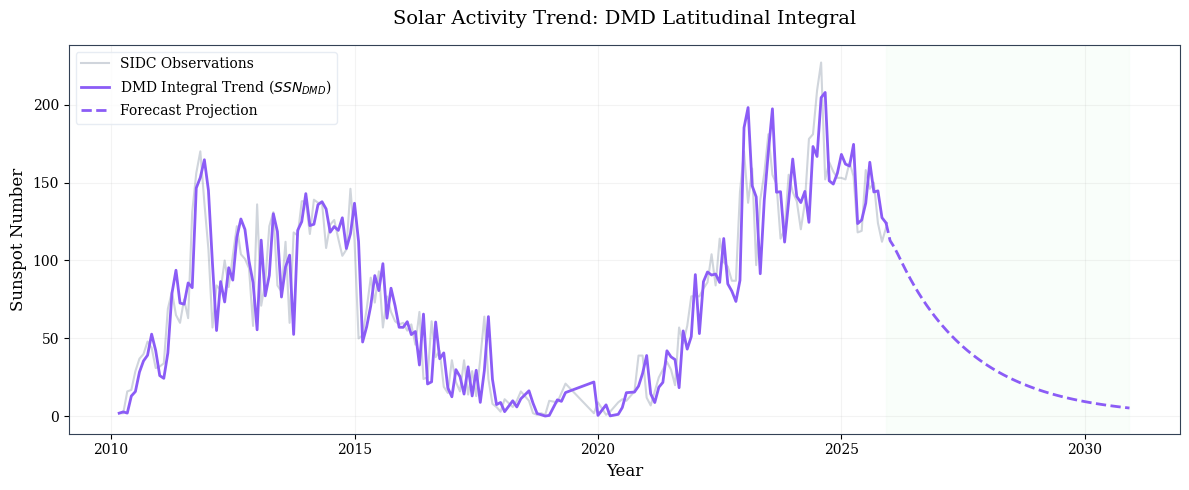
\includegraphics[width=0.92\textwidth]{figures/pred/dmd.png}
    \caption{Ajuste y predicción del número de manchas solares derivada de la
    integral latitudinal del modelo DMD ($\mathrm{SSN}_{\mathrm{DMD}}$). Las
    líneas punteadas corresponden a la predicción. \textbf{Fuente:} Elaboración
    propia.}
    \label{fig:ssn-dmd-projection}
\end{figure}


\section{Arquitectura y despliegue de base de datos}

La persistencia de datos se organiza mediante una base relacional desplegada en
Supabase sobre PostgreSQL. Esta capa conserva tanto los datos derivados de la
etapa de entrenamiento como los nuevos registros capturados desde la Raspberry Pi
5. La base no se limita a almacenar imágenes; mantiene la relación entre
conjuntos de datos, discos solares completos, recortes de manchas, predicciones,
metadatos de observación y capturas operativas recientes.

La base de datos actúa como punto de unión entre las etapas anteriores y la
plataforma web. En ella confluyen las imágenes de origen, las etiquetas usadas
para entrenamiento, las inferencias del detector y del clasificador, y los
productos de observación generados durante la operación del prototipo. Esta
centralización evita que la trazabilidad dependa de archivos aislados y permite
reconstruir el historial completo de cada observación.

\begin{figure}[H]
    \centering
    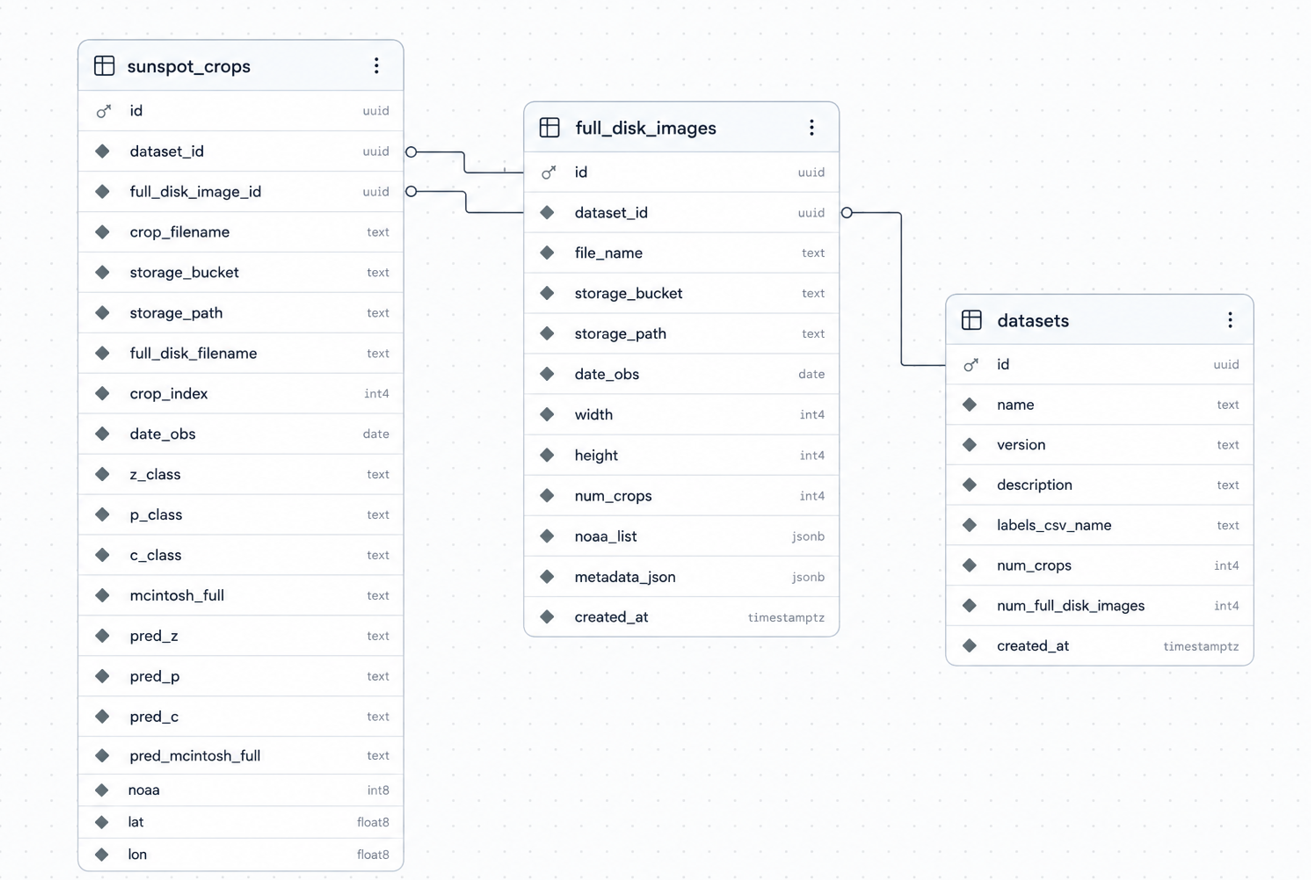
\includegraphics[width=0.95\textwidth]{figures/data/db_schema.png}
    \caption{Estructura relacional de la base de datos desplegada en Supabase.
    El esquema vincula conjuntos de datos, imágenes de disco completo, recortes
    de manchas solares y capturas recientes generadas desde la Raspberry Pi 5. \textbf{Fuente:} Elaboración propia.}
    \label{fig:db-structure-supabase}
\end{figure}


La arquitectura se apoya en tres tablas principales para los conjuntos
históricos. La tabla \texttt{datasets} identifica cada colección mediante un
\texttt{id} de tipo UUID, nombre, versión, descripción, archivo de etiquetas y
conteos generales de recortes e imágenes de disco completo. Esta entidad permite
separar versiones de datos, mantener trazabilidad sobre la procedencia de los
registros y evitar ambigüedades cuando se incorporan nuevos conjuntos.

La tabla \texttt{full\_disk\_images} almacena las imágenes de disco completo
asociadas a un \texttt{dataset}. Para cada imagen se registra el nombre del
archivo, el \textit{bucket} de almacenamiento, la ruta del objeto, la fecha de
observación, dimensiones, número de recortes asociados, lista NOAA y metadatos en
formato \texttt{jsonb}. Esta tabla funciona como punto de enlace entre la imagen
solar completa y las regiones activas extraídas a partir de ella.

Los recortes individuales se almacenan en \texttt{sunspot\_crops}. Esta tabla
contiene la referencia al conjunto de datos y a la imagen de disco completo, el
nombre y ruta del recorte, el índice de recorte, la fecha de observación, las
etiquetas reales $Z$, $P$, $C$, la combinación McIntosh completa, las predicciones
del modelo, la identificación NOAA, coordenadas heliográficas, longitud de
Carrington, extensión, área, clase magnética, número de manchas reportado por
SRD, tamaño original del recorte, confianza YOLO y centro de la detección en
píxeles. Con ello, cada recorte conserva simultáneamente información visual,
taxonómica, geométrica y operacional.

El esquema incorpora restricciones de unicidad para preservar consistencia. Por
ejemplo, \texttt{datasets} evita repetir una misma combinación de nombre y
versión; \texttt{full\_disk\_images} impide duplicar archivos dentro de un mismo
conjunto y rutas de almacenamiento; \texttt{sunspot\_crops} evita repetir nombres
de recortes por conjunto, rutas de objetos y pares \texttt{full\_disk\_image\_id}
-- \texttt{crop\_index}. Además, las claves foráneas utilizan eliminación en
cascada, por lo que al retirar un conjunto de datos también se eliminan sus
imágenes y recortes asociados, manteniendo integridad referencial.

Para facilitar consultas frecuentes se definen índices sobre identificadores de
conjunto, fecha de observación, imagen de disco completo, número NOAA y
clasificación McIntosh completa. Estos índices son relevantes para operaciones
como recuperar todos los recortes de una fecha, buscar regiones asociadas a una
NOAA específica, filtrar por combinación Zurich--McIntosh o reconstruir el
historial de una imagen de disco completo.

Las claves foráneas, restricciones de unicidad e índices sobre fecha,
identificador de conjunto, imagen de disco completo, NOAA y clasificación
McIntosh permiten reconstruir la trazabilidad de cada observación y acelerar
consultas frecuentes. Los archivos se conservan en Supabase Storage, incluyendo
el \textit{bucket} privado \texttt{snapshots}, mientras que PostgreSQL almacena
las rutas y metadatos necesarios para su recuperación. La tabla
\texttt{live\_captures} utiliza seguridad a nivel de fila, lo que permite
controlar el acceso desde la plataforma web sin perder la capacidad de consulta y
sincronización.

\section{Plataforma web}

La plataforma web constituye la capa de interacción del sistema. Su función es
convertir los datos persistidos y los modelos desplegados en herramientas de
consulta, visualización e inferencia accesibles para el usuario. Así, el flujo
iniciado con la construcción de datos y el entrenamiento de modelos culmina en
una interfaz capaz de mostrar observaciones, resultados taxonómicos, capturas
recientes y productos predictivos.

\subsection{Desarrollo en Next.js con despliegue en Vercel}

La plataforma web se implementa con Next.js y se despliega en
Vercel como interfaz centralizada para gestión, consulta y análisis de
observaciones solares. Este entorno complementa el procesamiento en el borde
realizado por la Raspberry Pi 5, aportando trazabilidad histórica, visualización
de resultados y acceso remoto. La persistencia y seguridad se apoyan en
Supabase, que gestiona autenticación, metadatos y almacenamiento de
productos derivados.

La arquitectura mantiene separación de responsabilidades en los siguientes
niveles:
\begin{itemize}
    \item Capa de interfaz: Componentes reactivos diseñados para la visualización dinámica de imágenes de disco solar y resultados de inferencia.
    \item Capa de datos y servicios: Módulos de comunicación con la base de datos PostgreSQL para consultas históricas y generación de informes de observación.
    \item Módulos de inferencia: Implementación de motores de ejecución para modelos ONNX directamente en el lado del cliente (navegador).
    \item Visualización predictiva: Herramientas gráficas para el análisis de la distribución latitudinal de manchas (diagramas de mariposa) y la evolución temporal del número de manchas solares (SSN).
\end{itemize}

El sistema opera bajo un esquema híbrido: la adquisición y el preprocesamiento se
ejecutan en el nodo de observación, mientras que la plataforma web mantiene la
disponibilidad remota, la consulta histórica y el soporte a la interpretación
científica.

\label{sec:web}


\subsection{Conversión y despliegue de modelos de procesamiento de imagen a ONNX para inferencia local en el dispositivo}

Los modelos de detección y clasificación se convierten al formato ONNX
(\textit{Open Neural Network Exchange}) para desacoplar la inferencia del entorno
de entrenamiento. Una vez exportados, pueden ejecutarse sin depender de PyTorch,
preservando la estructura computacional y los parámetros aprendidos. Esta
interoperabilidad facilita el despliegue en servidores ligeros, aplicaciones de
escritorio, dispositivos embebidos y navegadores web mediante ONNX
Runtime Web.

En el caso del detector YOLO26n, la entrada del modelo corresponde a una imagen
de disco solar completo previamente normalizada y redimensionada al tamaño
requerido por la red. Para el clasificador jerárquico basado en ConvNeXtV2 Atto, la
entrada consiste en recortes individuales de regiones activas ajustados a
$224 \times 224$ píxeles. La variante Atto se emplea para favorecer una
exportación íntegra desde PyTorch hacia ONNX, mientras que los salidales MLP
conservan el aprendizaje jerárquico de $Z$, $P$ y $C$. En ambos casos, la
exportación conserva la forma del tensor de entrada, el orden de canales, los
factores de normalización y la estructura exacta de las salidas.

Cada modelo exportado se valida comparando sus predicciones con las del entorno
original. Esta verificación confirma la consistencia numérica de la conversión y
permite detectar incompatibilidades de preprocesamiento, dimensiones, orden de
canales o lectura de salidas.

El despliegue \textit{on-device} consiste en ejecutar la inferencia directamente
en el dispositivo del usuario o en el nodo local de observación, evitando que
cada imagen deba enviarse a un servidor remoto para su procesamiento. En la
plataforma desarrollada, esta estrategia permite que los modelos ONNX se
ejecuten dentro del navegador web mediante la biblioteca ONNX Runtime Web. 
Este motor de inferencia utiliza WebAssembly (WASM) para la ejecución 
eficiente en CPU y la API de WebGPU (o WebGL como alternativa) para la 
aceleración por hardware, permitiendo realizar la inferencia localmente con 
un rendimiento cercano al nativo.

Operativamente, esta decisión reduce latencia, ancho de banda y dependencia de
servicios externos de inferencia. Aunque el procesamiento se ejecuta localmente,
los resultados se almacenan junto con imágenes y metadatos observacionales,
manteniendo trazabilidad y permitiendo consulta, revisión y comparación posterior
desde la plataforma web.